
%% Copyright 2019-2024 Elsevier Ltd
%% 
%% This file is part of the 'CAS Bundle'.
%% --------------------------------------
%% 
%% It may be distributed under the conditions of the LaTeX Project Public
%% License, either version 1.3c of this license or (at your option) any
%% later version.  The latest version of this license is in
%%    http://www.latex-project.org/lppl.txt
%% and version 1.3c or later is part of all distributions of LaTeX
%% version 1999/12/01 or later.
%% 
%% The list of all files belonging to the 'CAS Bundle' is
%% given in the file `manifest.txt'.
%% 
%% Template article for cas-sc documentclass for
%% single column output.

\documentclass[a4paper,fleqn]{cas-sc}

% If the frontmatter runs over more than one page
% use the longmktitle option.

%\documentclass[a4paper,fleqn,longmktitle]{cas-sc}

\usepackage[numbers]{natbib}
%\usepackage[authoryear]{natbib}
%\usepackage[authoryear,longnamesfirst]{natbib}
\usepackage{graphicx}
\usepackage{booktabs}
\usepackage{array}
\usepackage{algorithm}
\usepackage{algpseudocode}
\usepackage{enumitem}   
\usepackage{placeins}

%%%Author macros
\def\tsc#1{\csdef{#1}{\textsc{\lowercase{#1}}\xspace}}
\tsc{WGM}
\tsc{QE}
%%%

\begin{document}
\let\WriteBookmarks\relax
\def\floatpagepagefraction{1}
\def\textpagefraction{.001}

% Short title
\shorttitle{TE-Q-Transformer for Battery SOH Estimation}

% Short author
\shortauthors{ZA Lisan et~al.}

% Main title of the paper
\title[mode=title]{TE-Q-Transformer: A Temperature-Embedded Quantum Framework for Battery State-of-Health Estimation}

% First author
\author[1]{Zadid Al Lisan}[orcid=0009-0001-1801-051X]
\ead{lisan15-5426@diu.edu.bd}

\author[1]{Md. Sulyman Islam Sifat}[orcid=0009-0005-6377-8973]

\ead{sifat15-4004@diu.edu.bd}

\author[3]{M.S. Hossain Lipu}[orcid=0000-0001-9060-4454] % replace XXXX with correct last 4 digits
\ead{molla_lipu@uow.edu.au}


\author[2]{Nazakat Ali}[orcid=0000-0002-3875-812X] % replace XXXX with correct last 4 digits
\ead{nazakat.ali@se.abb.com}



\author[1]{Md Alamgir Kabir}[orcid=0000-0002-7136-6339]
\ead{kabir.cse@diu.edu.bd}
\cormark[1]
%\credit{Conceptualization, Project administration, Writing – review \& editing, Supervision}

\affiliation[1]{organization={Department of Computer Science and Engineering, Daffodil International University},
            city={Dhaka},
            country={Bangladesh}}

\affiliation[2]{organization={ABB},
    city={Vasteras},
    country={Sweden}}

\affiliation[3]{organization={School of Electrical, Computer and Telecommunications Engineering, University of Wollongong},
    city={New South Wales 2522},
    country={Australia}}

    
% Corresponding author text
\cortext[1]{Corresponding author}
% Footnote text
\fntext[1]{}

\begin{abstract}
Reliable state-of-health estimation is essential for the safe and efficient operation of lithium-ion batteries in electric vehicles and energy storage systems. Operating temperature strongly affects battery aging. However, existing data-driven models simply treat temperature as an ordinary numerical input, ignoring the underlying physical degradation kinetics. As a result, these models often struggle to generalize across different, unseen cells. To address this, we introduce TE-Q-Transformer, a hybrid framework that integrates Arrhenius-based kinetics for high-temperature solid electrolyte interphase growth and low-temperature lithium plating into a four-qubit simulated quantum circuit and a Conv1D-Transformer backbone. Evaluated on the NASA cross-cell benchmark, TE-Q-Transformer achieves a macro RMSE of 0.0168 and an $R^2$ of 0.870, outperforming ten contemporary baselines. Controlled ablations show that the physics-guided encoding reduces macro RMSE from 0.0201 to 0.0168 (a 16.5\% improvement) over conventional temperature scaling, while replacing the quantum circuit with a parameter-matched classical counterpart raises the error to 0.0431. These results demonstrate that embedding degradation kinetics directly into input features substantially improves cross-cell state-of-health estimation. Source code is available at \href{https://github.com/LisanHub/Te-Q-Transformer}{https://github.com/LisanHub/Te-Q-Transformer}.
\end{abstract}

% Research highlights
% \begin{highlights}
% \item We propose TE-Q-Transformer, a hybrid quantum-classical model for battery SOH estimation.
% \item An Arrhenius-informed quantum gate embeds thermal ageing physics directly into the model.
% \item The model gives the best cross-battery accuracy on the non-linear NASA dataset.
% % \item A fair NASA benchmark with a multi-temperature cross-cell held-out split is reported against five baseline models. The model is further validated on the CALCE dataset.
% \item The model is further validated on the CALCE dataset, where it again achieves the lowest RMSE and MAE and the highest $R^2$ among six models.
% \end{highlights}

% Keywords
\begin{keywords}
Quantum machine learning \sep Battery state of health \sep Hybrid quantum-classical model \sep Transformer \sep Arrhenius temperature encoding
\end{keywords}

\maketitle

% Main text
% Main text
\section{Introduction}\label{sec:intro}

Lithium-ion batteries play a central role in electric vehicles and stationary energy storage systems because of their high energy density, long cycle life, and declining cost \citep{ralls2023role}. Reliable and safe battery operation depends on the battery management system (BMS), which monitors operational signals including voltage, current, and temperature to maintain cell operation within safe limits \citep{ali2025comprehensive}. During repeated cycling, batteries experience progressive degradation through electrochemical mechanisms that cause capacity loss and internal resistance growth \citep{li2025deep}. To track this degradation over successive operating cycles, battery state of health (SOH) is estimated from measured operating data. In this study, SOH is defined as the ratio of the discharge capacity at a given cycle to the initial discharge capacity of that cell. Accurate SOH estimation is essential for ensuring operational safety, extending service life, and guiding battery replacement or second-life deployment.

Operating temperature strongly affects lithium-ion battery degradation. Temperature is not merely an external operating condition; it influences the chemical and electrochemical reaction kinetics that contribute to capacity fade. At elevated temperatures, thermally activated parasitic side reactions between the electrolyte and active materials accelerate, promoting solid electrolyte interphase (SEI) growth and solvent decomposition \citep{gao2023effect}. Conversely, at sub-ambient temperatures, the kinetics of lithium-ion transport and solid-state diffusion slow down, increasing charge-transfer resistance and inducing electrode polarization; under charging conditions, this polarization can cause metallic lithium plating on the negative electrode \citep{kumar2024}. Consequently, different degradation pathways become important across operating temperatures. Temperature therefore influences the rate and trajectory of health degradation in a mechanism-dependent manner.

To capture dynamic degradation trajectories, data-driven models, particularly deep sequential architectures, have increasingly been adopted for battery SOH estimation from measured voltage, current, and temperature time series \citep{sohtec2024}. In conventional data-driven formulations, temperature is commonly supplied as an additional numerical input channel transformed through standard linear scaling or normalization procedures \citep{zhao2025capacity,tcntransformer2025}. Although feature normalization adjusts numerical magnitudes, it does not explicitly represent the underlying temperature-dependent degradation kinetics. At the same time, battery cells exhibit inherent cell-to-cell variation arising from manufacturing differences and operating history \citep{lu2024mechanisms}. Models trained on a specific set of cells can show degraded performance when applied to previously unseen cells. Furthermore, random cycle-level train-test partitioning can introduce optimistic evaluation bias through temporal leakage across adjacent operating cycles, making fixed held-out-cell evaluation important for assessing cross-cell generalization \citep{sedlavrik2025advanced}.

To incorporate physical knowledge into data-driven SOH estimation, physics-guided methods use equivalent circuit models, physics-derived features, or loss-function regularization \citep{chen2023state,pepe2023}. While these methods introduce physical information, the reviewed approaches generally do not transform the temperature input into a representation directly derived from degradation kinetics. In parallel, quantum machine learning has recently been explored for battery SOH estimation, using parameterized quantum circuits as non-linear feature transformation layers that interface with classical neural networks \citep{komarsofla2026,liang2025stochastic}. However, the reviewed battery QML studies do not describe a temperature representation explicitly derived from degradation kinetics. While recent perspectives have highlighted the integration of physics-guided modeling with quantum machine learning as an emerging direction in battery prognostics \citep{piqml2026}, whether embedding degradation kinetics directly into feature representations improves SOH estimation has not been systematically evaluated. These considerations motivate the central scientific question investigated in this work: can physics-guided temperature encoding, rather than conventional temperature feature processing, improve lithium-ion battery SOH estimation under cross-cell generalization?

To address this question, this work introduces TE-Q-Transformer, a hybrid framework that encodes temperature according to degradation kinetics and transforms multi-channel battery measurements through a parameterized entangling quantum circuit. The resulting features are processed by a temporal architecture combining local convolution with Transformer self-attention and evaluated under fixed held-out-cell protocols. This framework therefore evaluates whether physics-guided temperature encoding improves estimation accuracy and cross-cell generalization compared with conventional temperature processing under identical temporal modeling and evaluation protocols.

The main contributions of this paper are summarized as follows:
\begin{enumerate}[label=(\roman*)]
\item \textbf{Physics-guided temperature representation:} We formulate a temperature encoding that embeds degradation kinetics into the feature representation, representing distinct thermal aging mechanisms, including elevated-temperature SEI growth and sub-ambient lithium plating, before quantum feature mapping and temporal sequence modeling, rather than treating temperature as an ordinary numerical channel.
\item \textbf{Controlled component analysis:} We use controlled ablations to separate the effects of physics-guided temperature encoding, the individual degradation mechanisms, the quantum feature mapping, and the main temporal architecture components. A near-parameter-matched classical counterpart is used to assess the contribution of the quantum representation under the same physics-guided encoding and temporal backbone.
\item \textbf{Cross-cell and external evaluation:} We evaluate TE-Q-Transformer under a fixed NASA held-out-cell protocol covering unseen-cell generalization and short temporal extrapolation, with CALCE CS2 cells used as an external zero-shot test of the NASA-trained model.
\end{enumerate}

The remainder of this paper is organized as follows. Section~\ref{sec:related} reviews related work on data-driven battery SOH estimation, physics-guided approaches, and quantum machine learning. Section~\ref{sec:method} details the methodology of TE-Q-Transformer, including problem formulation, physics-guided temperature encoding, quantum circuit design, and temporal network architecture. Section~\ref{sec:experiments} presents the experimental setup, NASA cross-cell evaluation results, baseline comparisons, ablation studies, and external zero-shot evaluation on CALCE cells. Section~\ref{sec:conclusion} concludes the paper and outlines directions for future research.




\section{Related Work}\label{sec:related}

\subsection{Data-driven Battery SOH Estimation}\label{sec:rw-data}
While physics-based electrochemical models provide detailed insight into internal cell dynamics, their governing parameters are difficult to identify and calibrate for practical onboard implementation \citep{asiri2025}. Consequently, data-driven approaches have gained prominence by learning non-linear mappings directly from measured battery operating signals, such as voltage, current, and temperature time series \citep{zhao2025capacity,wang2026lithium}. Because battery degradation is path-dependent and cumulative operating history influences future fade, sequential learning architectures are particularly suited for tracking multi-cycle health trajectories.

Early data-driven investigations relied on classical statistical regression and machine learning algorithms, such as support vector regression, Gaussian process regression, and random forests \citep{zhao2022lithium}. However, many of these methods rely on handcrafted health indicators extracted from partial charging or discharging curves, which can discard informative temporal correlations \citep{wang2024state}. To capture dynamic degradation patterns from sequential battery measurements, deep recurrent neural networks, including long short-term memory (LSTM) and gated recurrent unit (GRU) architectures, were subsequently adopted to track temporal dependencies in battery degradation sequences. For example, Li et al. \citep{li2023} combined temporal convolutional networks with LSTM units to capture multi-scale dependencies in degradation records, while Quan et al. \citep{qhdbo2025} integrated bidirectional temporal convolutions with bidirectional GRUs to extract degradation features under complex operational profiles. Similarly, Guo et al. \citep{guo2023} applied gated recurrent units with time-series filtering to track capacity degradation, and Wen et al. \citep{wen2024lithium} implemented an interpretable boosting framework to isolate critical degradation segments from real-world electric vehicle charging data. While these recurrent and convolutional models capture sequential dependencies effectively, recurrent architectures process time steps sequentially, which can make modeling long-range dependencies more difficult over extended intra-cycle sequences.

To address the challenges of sequential recurrent processing, attention mechanisms and Transformer networks have increasingly been adopted for battery sequence modeling. Self-attention allows interactions between different time steps across the sequence in parallel, allowing models to capture long-range temporal dependencies regardless of the temporal distance between measurement points. For instance, Gu et al. \citep{cnn_transformer2023} developed a hybrid CNN-Transformer architecture, utilizing convolutional layers to extract local temporal features before passing sequence representations to a Transformer encoder for state-of-health estimation. Chen et al. \citep{tcntransformer2025} fused temporal convolutional networks with Transformer layers to monitor battery pack aging across extended vehicle operating periods. In a related direction, Gui et al. \citep{gui2025multi} proposed a parallel CNN-Transformer network with multi-modal information alignment, showing that local convolutional feature extraction and global self-attention provide complementary temporal representations for battery sequence analysis. Furthermore, Sun et al. \citep{sun2025battery} incorporated attention mechanisms into gradient boosting to extract dynamic health indicators from driving cycles. These studies show that local temporal convolutions and global self-attention can be used together to model both short- and long-range patterns in multi-channel battery time series.

Despite the progress in deep sequential modeling, generalization across different battery cells remains an open challenge. Battery degradation can vary across cells because of manufacturing variation and differences in operating conditions \citep{lu2024mechanisms}. Consequently, models trained on a specific set of cells may show degraded performance when applied to unseen test cells. Sedla{\v{r}}{\'\i}k et al. \citep{sedlavrik2025advanced} demonstrated that random train-test cycle partitioning can introduce optimistic bias through information leakage across adjacent cycles, showing that strict held-out cell protocols provide a more appropriate setting for assessing transfer to previously unobserved cells. To improve cross-cell generalization, transfer learning frameworks have been explored; for example, Sahoo et al. \citep{sahoo2022transfer} developed a transfer learning methodology to adapt pre-trained neural networks across different battery cells and operating conditions. These findings support the use of fixed held-out cell protocols when evaluating transfer to previously unobserved cells.

In conventional empirical SOH formulations, temperature is commonly included as a numerical input feature and normalized before model training \citep{sohtec2024,liu2025multi}. Such preprocessing changes the numerical range of temperature but does not explicitly encode the kinetic relationships underlying temperature-dependent degradation.

\subsection{Physics-guided and Temperature-aware SOH Estimation}\label{sec:rw-physics}
The temperature dependence of lithium-ion battery degradation arises from distinct thermally activated electrochemical pathways that contribute to capacity loss and impedance rise. At elevated temperatures, accelerated parasitic side reactions between the electrolyte and active materials promote solid electrolyte interphase (SEI) growth on the negative electrode and solvent decomposition \citep{gao2023effect}. Conversely, at sub-ambient temperatures, retarded lithium-ion desolvation and solid-state diffusion increase charge-transfer resistance and induce electrode polarization \citep{yang2018understanding}; under low-temperature charging, negative-electrode potentials can drop below zero volts relative to $\mathrm{Li/Li}^+$, inducing metallic lithium plating \citep{kumar2024}. Consequently, degradation behavior can differ substantially between elevated and sub-ambient temperatures relative to moderate conditions \citep{waldmann2014temperature}.

To account for these mechanistic behaviors, recent research has explored physics-guided machine learning for battery SOH estimation. Rather than treating neural networks as purely empirical regressors, physics-guided frameworks introduce physical knowledge through several distinct strategies. One strategy couples neural networks with equivalent circuit models and uses identified circuit parameters as additional inputs for SOH estimation \citep{chen2023state}. A second strategy relies on physics-derived feature engineering, wherein degradation indicators, such as peak positions and areas from incremental capacity and differential voltage curves, are extracted prior to sequence modeling \citep{pepe2023}. Another strategy uses physics-informed neural networks that incorporate governing differential equations or empirical degradation laws directly into the loss function during optimization \citep{chen2025pinn}.

Recent studies have incorporated temperature-dependent aging relationships into SOH estimation under different operating conditions. The Arrhenius relationship is commonly used to describe thermally activated reaction rates in chemical kinetics. In battery degradation studies, Arrhenius expressions are used to describe how side-reaction rates scale with absolute temperature relative to activation energy barriers \citep{kucinskis2022arrhenius}. Building on this principle, Kumar et al. \citep{kumar2026temperature} developed a temperature- and impedance-aware LSTM-PINN, incorporating Arrhenius kinetics, impedance growth, and monotonicity constraints into the loss function to mitigate non-physical SOH trajectory drift on NASA battery records. Similarly, Yang et al. \citep{yang2025physics} formulated a multi-task physics-informed framework that couples physical degradation boundaries with Transformer sequence learning to co-estimate SOH, remaining useful life, and degradation paths. In related studies, Chen et al. \citep{chen2025pinn} implemented physics-informed regularization for small-sample degradation scenarios, while Fan et al. \citep{fan2025spatiotemporal} employed a spatiotemporal graph attention network to handle domain shifts across distinct operating temperature scenarios. Together, these studies incorporate temperature and physical information through different forms of model coupling, loss regularization, and temperature-aware feature learning.

Although these frameworks incorporate physical knowledge into SOH estimation, they generally introduce physical information through external constraints rather than direct input transformations. In physics-informed formulations, governing relationships are enforced through auxiliary loss penalties that regularize network training, while the network continues to receive measured variables through conventional numerical channels \citep{yang2025physics}. Similarly, two-stage decoupled frameworks reconstruct internal states before sequence modeling without modifying the underlying feature encoding \citep{li2025unified}. Furthermore, existing temperature-aware frameworks predominantly focus on elevated-temperature Arrhenius acceleration, while explicit representations of sub-ambient degradation mechanisms, such as lithium plating, remain less common in sequential architectures \citep{kumar2026temperature,fan2025spatiotemporal}. This creates a clear representation-level gap: embedding both high- and low-temperature degradation kinetics directly into the input features prior to sequence modeling.

\subsection{Quantum Machine Learning for Battery SOH Estimation}\label{sec:rw-qml}
Quantum machine learning has recently been explored as a feature-transformation approach for battery state-of-health estimation \citep{komarsofla2026}. In hybrid quantum-classical configurations, parameterized quantum circuits map multi-channel sensor measurements into quantum state representations through parameterized rotations and entangling gates before passing transformed features to classical network layers \citep{biamonte2017,cerezo2021}.

Recent studies have applied hybrid quantum-classical architectures to battery SOH estimation. Wang and Kebede \citep{wang2026prediction} proposed a quantum long short-term memory (QLSTM) model with transfer learning to process charging sequences from electric vehicle battery packs. Soon and Soon \citep{soon2025hybrid} combined a quantum neural network with a classical gated recurrent unit (QNN-GRU) for battery SOH forecasting, using the quantum network as a feature transformation stage before temporal prediction. In another approach, Liang et al. \citep{liang2025stochastic} developed a quantum convolutional neural network (QCNN) with automated feature fusion, achieving lower estimation error than classical convolutional and multilayer perceptron baselines on battery degradation records. Furthermore, Monika and Sood \citep{monika2026multi} evaluated a hybrid QLSTM model across multiple battery datasets, while Wang et al. \citep{wang2024lithium} used variational quantum algorithms to optimize stacking ensemble weights for battery health prediction.

In these hybrid configurations, the quantum circuit functions as a non-linear feature transformation stage prior to classical temporal processing. Typical implementations employ angle encoding to map classical inputs to qubit rotation angles, followed by parameterized entangling operations and expectation-value measurements \citep{cerezo2021}. To improve encoding flexibility, Ovalle-Magallanes et al. \citep{ovalle2023quantum} introduced learnable rotation parameters into angle encoding, demonstrating that trainable encoding gates enhance feature representation in hybrid quantum-classical models.

Despite these advances, existing battery QML studies leave critical methodological questions unresolved. First, when temperature is incorporated into hybrid quantum models, it is treated as a standard numerical channel rather than being transformed according to degradation kinetics. Second, existing investigations rarely benchmark parameterized quantum circuits against classical counterparts with closely matched parameter counts under identical temporal backbones and held-out-cell protocols. While recent perspectives highlight physics-informed quantum machine learning as an emerging direction for battery prognostics \citep{piqml2026}, systematic evaluations of kinetics-derived feature representations under cross-cell evaluation remain unaddressed.

In synthesis, the reviewed literature reveals three converging insights across data-driven sequence modeling, physics-guided methods, and quantum machine learning. Sequential architectures model battery degradation trajectories effectively, while physics-guided methods introduce physical knowledge through model coupling, derived features, or training constraints. However, temperature is still predominantly processed as a numerical input rather than a kinetics-derived representation, and existing battery QML studies do not explicitly integrate temperature-dependent degradation mechanisms. This representation-level gap motivates the central scientific question investigated in this study: can physics-guided temperature encoding, rather than conventional temperature feature processing, improve lithium-ion battery SOH estimation under cross-cell generalization?













\section{Methodology}\label{sec:method}

This section presents the mathematical formulation and architecture of TE-Q-Transformer for battery state-of-health estimation. The presentation is organized into seven parts. Section~\ref{sec:problem} defines the cycle-level state-of-health estimation problem. Section~\ref{sec:overview} provides an architectural overview of the framework and introduces its three core design features. Section~\ref{sec:temp_encoding} details the physics-guided temperature encoding, including the Arrhenius kinetic terms and their analytical temperature sensitivity. Section~\ref{sec:quantum_mapping} presents the four-qubit variational circuit, the rich entanglement topology, and the bounded quantum readout. Section~\ref{sec:temporal_modeling} describes the latent projection, local temporal convolution, Transformer encoder, regression head, and the exact parameter count breakdown. Section~\ref{sec:optimization} defines the training objective and the end-to-end optimization algorithm. Finally, Section~\ref{sec:workflow} summarizes the complete operational workflow and connects the methodology to the experimental evaluations in Section~\ref{sec:experiments}.

\subsection{Problem Formulation}\label{sec:problem}

Consider a lithium-ion battery cell operating under repeated charge and discharge cycling. In battery health prognostics, the state of health, denoted SOH, at cycle $i$ is defined as the ratio of the discharge capacity $C_i$ to the initial discharge capacity $C_0$:
\begin{equation}
\mathrm{SOH}_i = \frac{C_i}{C_0}.
\label{eq:soh_def}
\end{equation}
Here, $i$ is the cycle index, $C_i$ is the discharge capacity measured at cycle $i$, and $C_0$ is the baseline discharge capacity measured during the first cycle of that cell. The calculated SOH serves as the scalar target that the model predicts for each discharge cycle.
Each discharge cycle is monitored through synchronized sensor observations. For cycle $i$, the measurements are arranged as a multivariate sequence matrix of length $L = 512$ with four physical feature channels:
\begin{equation}
X_i =
\begin{bmatrix}
\mathbf{x}_{i,1}^{\top} \\
\mathbf{x}_{i,2}^{\top} \\
\vdots \\
\mathbf{x}_{i,L}^{\top}
\end{bmatrix}
\in \mathbb{R}^{L \times 4},
\label{eq:input_seq}
\end{equation}
where each row corresponds to the observation vector $\mathbf{x}_{i,\ell} \in \mathbb{R}^4$ at time index $\ell \in \{1, \dots, L\}$:
\begin{equation}
\mathbf{x}_{i,\ell} = \bigl[V_{i,\ell},\, I_{i,\ell},\, T_{i,\ell},\, t_{\mathrm{norm},i,\ell}\bigr]^{\top}.
\label{eq:input_obs}
\end{equation}
Here, $V_{i,\ell}$ is the terminal voltage, $I_{i,\ell}$ is the load current, $T_{i,\ell}$ is the measured cell surface temperature in degrees Celsius, and $t_{\mathrm{norm},i,\ell} \in [0, 1]$ is the normalized intra-cycle time. The normalized time is obtained by dividing the elapsed time since the beginning of discharge by the total duration of that discharge cycle.

The objective of the model is to learn a parameterized nonlinear mapping $f_{\Theta}: \mathbb{R}^{L \times 4} \to \mathbb{R}$ that estimates the cycle SOH from the discharge sequence:
\begin{equation}
\hat{y}_i = f_{\Theta}(X_i),
\label{eq:mapping}
\end{equation}
where $\hat{y}_i$ is the predicted SOH and $\Theta$ denotes the complete set of trainable parameters. Given a training dataset of $N$ sequence-target pairs, denoted $\{(X_i, y_i)\}_{i=1}^N$ with reference values $y_i = \mathrm{SOH}_i$, model training corresponds to finding the optimal parameter set $\Theta^*$ that minimizes an empirical discrepancy function $\mathcal{L}$:
\begin{equation}
\Theta^* = \arg\min_{\Theta} \frac{1}{N}\sum_{i=1}^N \mathcal{L}\bigl(y_i,\, f_{\Theta}(X_i)\bigr).
\label{eq:opt_goal}
\end{equation}
The discrepancy function $\mathcal{L}$ evaluates the error between the reference target $y_i$ and the prediction $\hat{y}_i$. In Section~\ref{sec:optimization}, this objective is instantiated as the mean squared error loss for end-to-end optimization.

\subsection{Overview of the Proposed TE-Q-Transformer}\label{sec:overview}

\begin{figure}[t]
  \centering
  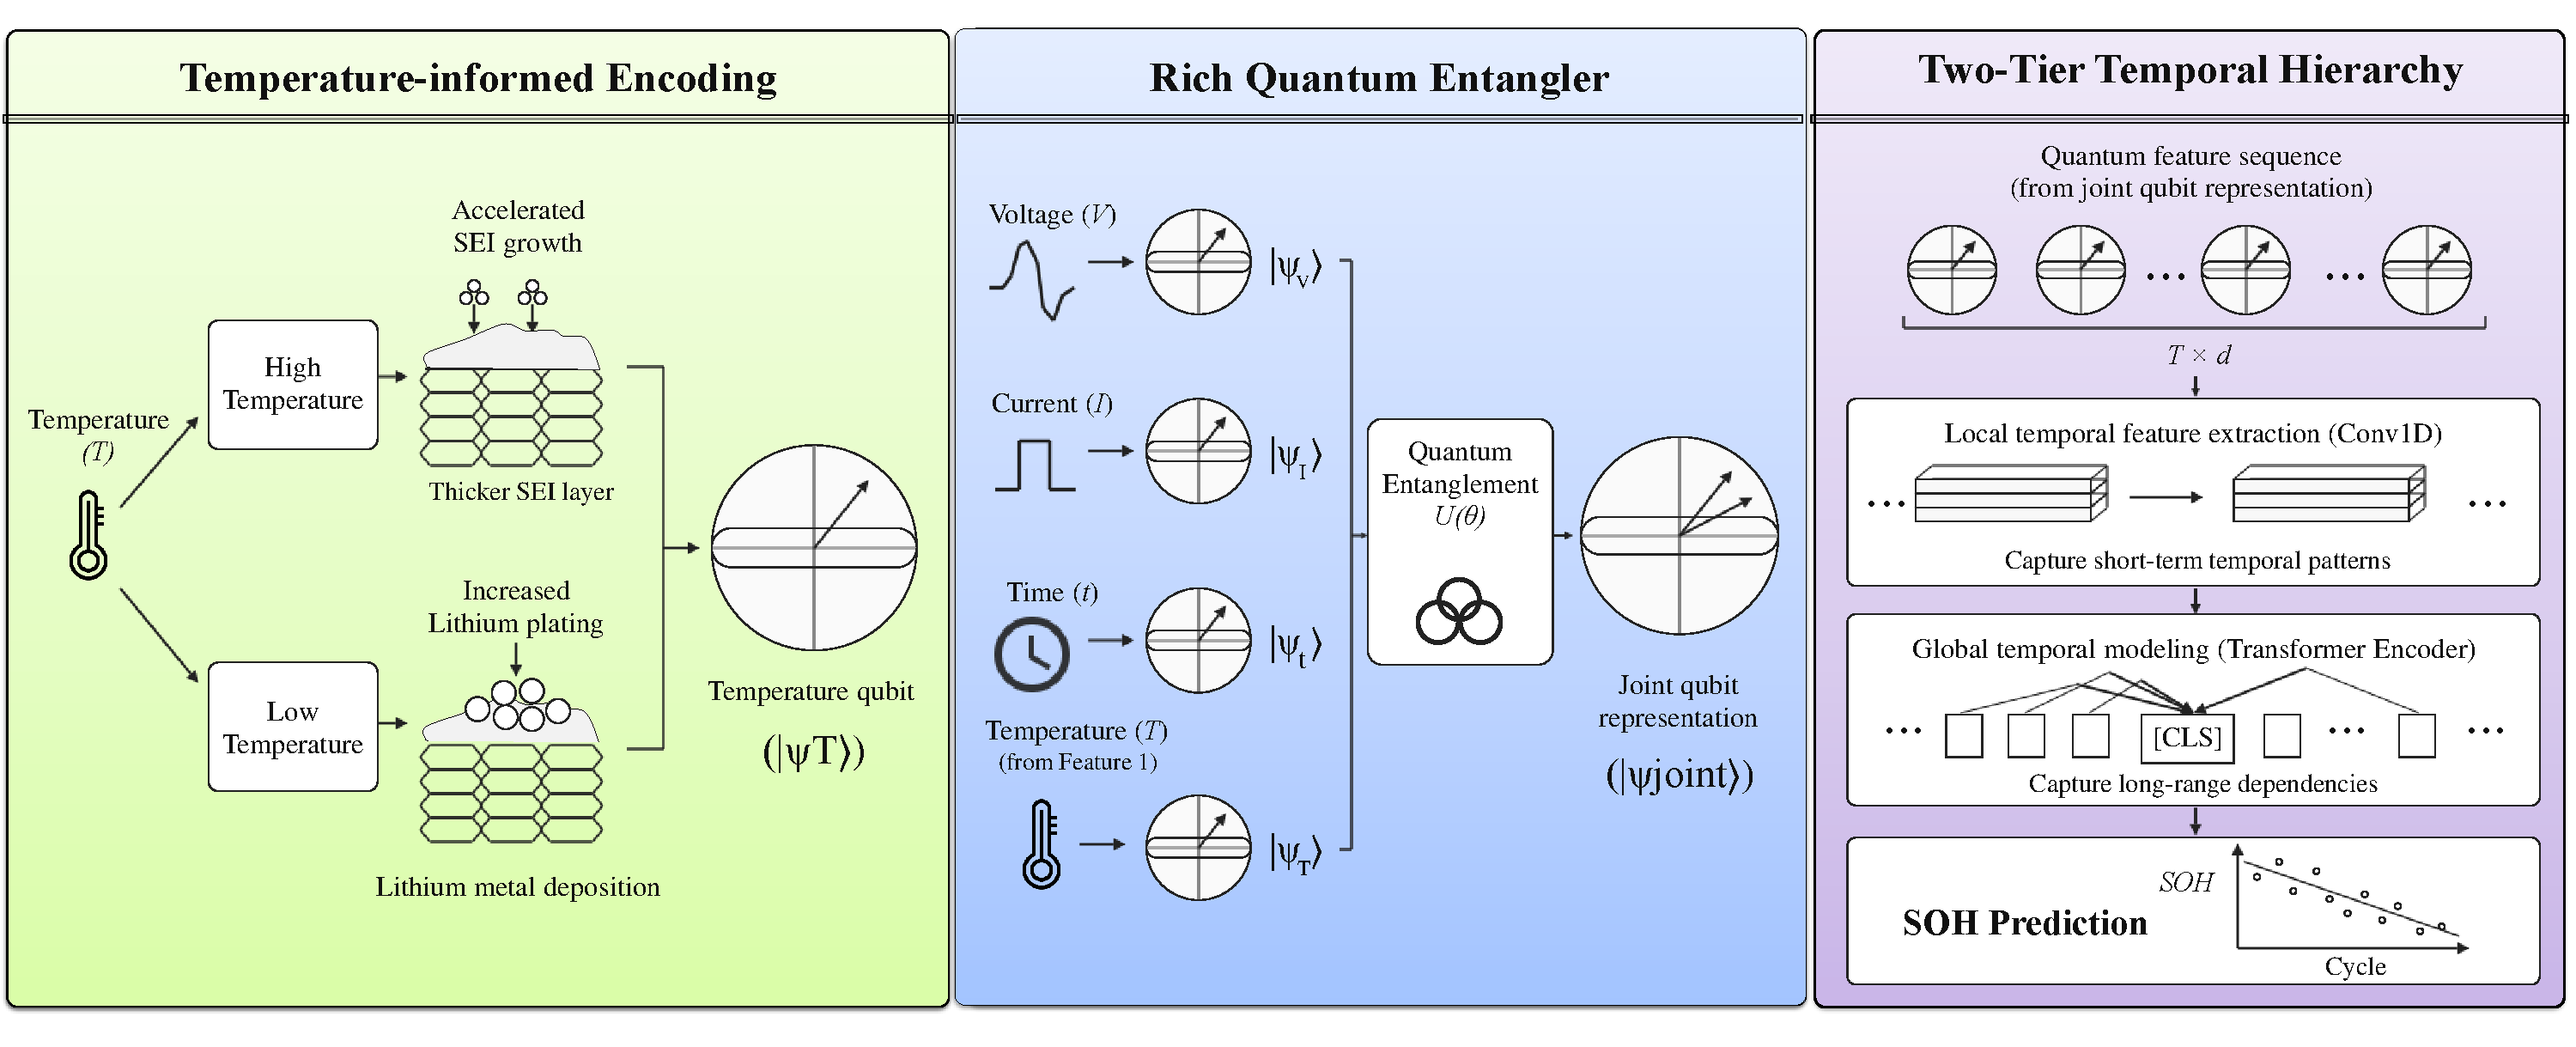
\includegraphics[width=\linewidth]{figs/TE-Q-TRANSFORMER_Features.pdf}
  \caption{Core design features of the proposed TE-Q-Transformer framework: (a)~physics-guided temperature encoding linking elevated-temperature SEI growth and low-temperature lithium plating to the temperature qubit state $|\psi_T\rangle$; (b)~rich parameterized quantum entangler mapping cross-channel interactions into a joint multi-qubit representation $|\psi_{\mathrm{joint}}\rangle$; and (c)~two-tier temporal hierarchy integrating local Conv1D feature extraction with global Transformer self-attention.}\label{fig:features}\label{fig1}
\end{figure}

When temperature is treated as an ordinary input feature, it is commonly normalized together with the other sensor channels using linear scaling. However, in lithium-ion batteries, operating temperature influences degradation through temperature-dependent kinetic processes that behave differently across operating regimes. High temperatures accelerate parasitic reaction rates, whereas low temperatures increase internal resistance and promote lithium plating. Linear scaling alone does not explicitly represent these opposing temperature-dependent kinetic effects. TE-Q-Transformer therefore combines physics-guided temperature encoding, quantum feature mapping, and hierarchical temporal modeling, as illustrated in Figure~\ref{fig:features}:

\begin{enumerate}[leftmargin=*,noitemsep,topsep=3pt]
\item \textbf{Physics-guided temperature encoding:} Rather than applying standard min--max normalization to temperature, the model evaluates solid electrolyte interphase (SEI) growth and lithium plating through two Arrhenius-inspired kinetic terms. These terms govern the rotation angle of a dedicated temperature qubit, representing temperature through degradation-related kinetics prior to quantum encoding.
\item \textbf{Rich quantum feature representation:} The four physical channels are mapped to four individual qubits in a quantum circuit. A parameterized entangling circuit that includes single-qubit rotations, controlled-NOT gates, Ising $ZZ$ interactions, and Toffoli gates allows interactions among the encoded channels to be represented in an entangled multi-qubit state. Expectation values of Pauli-$Z$ operators then provide a bounded four-dimensional feature vector for each time step.
\item \textbf{Two-tier temporal hierarchy:} The sequence of quantum features is projected into a latent space and processed at two complementary temporal scales. A one-dimensional convolutional layer first extracts local temporal patterns across adjacent time steps. A multi-head self-attention Transformer encoder then models long-range sequence dependencies across the full discharge cycle. A learnable $\mathrm{[CLS]}$ token aggregates sequence context for the final regression head.
\end{enumerate}

At each time step, the four input measurements are first mapped to a quantum feature vector. These vectors are then projected into a latent space and processed by the Conv1D layer. The resulting sequence is passed to the Transformer for global temporal modeling and SOH prediction. The temperature encoding is formulated mathematically in the next subsection.

\subsection{Physics-Guided Temperature Encoding}\label{sec:temp_encoding}

Temperature strongly affects battery degradation through temperature-dependent reaction kinetics. Different degradation mechanisms can become more important under different thermal conditions. At elevated temperatures, capacity fade is associated with accelerated solid electrolyte interphase (SEI) layer growth and parasitic solvent reduction on the negative electrode~\citep{waldmann2014temperature}. At sub-ambient temperatures, charge-transfer resistance rises and lithium solid-state diffusion slows, which can promote metallic lithium plating on the graphite anode~\citep{yang2018understanding}. TE-Q-Transformer uses two temperature-dependent kinetic terms based on the Arrhenius relationship to represent these different degradation tendencies.

\subsubsection{Temperature Conversion and Arrhenius Formulations}

Because the Arrhenius formulation uses absolute temperature, the measured cell surface temperature $T$ in degrees Celsius is converted to $T_K$ in Kelvin:
\begin{equation}
T_K = \max(T + 273.15,\, 1.0),
\label{eq:kelvin}
\end{equation}
where $273.15$ is the standard Celsius-to-Kelvin offset. The lower bound of $1.0\,\mathrm{K}$ serves as a numerical safeguard against non-positive values during execution. In all experimental cycles, the measured temperatures remain well above this boundary.

The Arrhenius formulation is defined relative to a reference temperature $T_{\mathrm{ref}} = 298.15\,\mathrm{K}$, corresponding to $25\,^\circ\mathrm{C}$, with universal gas constant $R = 8.314462618\,\mathrm{J\,mol^{-1}\,K^{-1}}$. The SEI kinetic factor $\phi_{\mathrm{sei}}$ is formulated as an Arrhenius expression relative to reference conditions~\citep{kucinskis2022arrhenius}:
\begin{equation}
\phi_{\mathrm{sei}} = \exp\!\left(\frac{10^4 E_{a,\mathrm{sei}}}{R}\left(\frac{1}{T_{\mathrm{ref}}} - \frac{1}{T_K}\right)\right),
\label{eq:arrhenius-sei}
\end{equation}
where $\phi_{\mathrm{sei}}$ denotes the SEI kinetic factor and $E_{a,\mathrm{sei}}$ is a trainable empirical parameter scaling the temperature sensitivity of high-temperature degradation. The multiplier $10^4$ is an implementation-level scaling factor applied to the trainable parameter in the Arrhenius exponent. For $E_{a,\mathrm{sei}} > 0$, $\phi_{\mathrm{sei}}$ increases with temperature above the reference temperature because $(1/T_{\mathrm{ref}} - 1/T_K) > 0$ when $T_K > T_{\mathrm{ref}}$.

To represent low-temperature degradation independently, a complementary kinetic factor $\phi_{\mathrm{pl}}$ is formulated for lithium plating. Because plating conditions worsen as temperature falls below the reference point, the difference of reciprocal temperatures is reversed:
\begin{equation}
\phi_{\mathrm{pl}} = \exp\!\left(\frac{10^4 E_{a,\mathrm{pl}}}{R}\left(\frac{1}{T_K} - \frac{1}{T_{\mathrm{ref}}}\right)\right),
\label{eq:arrhenius-pl}
\end{equation}
where $\phi_{\mathrm{pl}}$ denotes the plating kinetic factor and $E_{a,\mathrm{pl}}$ is a trainable empirical parameter for low-temperature kinetics. Similarly, for $E_{a,\mathrm{pl}} > 0$, $\phi_{\mathrm{pl}}$ increases as temperature falls below the reference temperature because $(1/T_K - 1/T_{\mathrm{ref}}) > 0$ when $T_K < T_{\mathrm{ref}}$.

\subsubsection{Analytical Temperature Sensitivity}

Differentiating the two kinetic factors with respect to absolute temperature $T_K$ yields their analytical temperature sensitivities:
\begin{align}
\frac{\partial \phi_{\mathrm{sei}}}{\partial T_K} &= \left(\frac{10^4 E_{a,\mathrm{sei}}}{R T_K^2}\right)\phi_{\mathrm{sei}}, \label{eq:dphi_sei} \\
\frac{\partial \phi_{\mathrm{pl}}}{\partial T_K} &= -\left(\frac{10^4 E_{a,\mathrm{pl}}}{R T_K^2}\right)\phi_{\mathrm{pl}}. \label{eq:dphi_pl}
\end{align}
Because $\phi_{\mathrm{sei}} > 0$ and $\phi_{\mathrm{pl}} > 0$ for all physical temperatures, the signs of these derivatives depend directly on the signs of the empirical parameters $E_{a,\mathrm{sei}}$ and $E_{a,\mathrm{pl}}$. Under the condition that $E_{a,\mathrm{sei}} > 0$ and $E_{a,\mathrm{pl}} > 0$, the partial derivatives satisfy:
\begin{equation}
\frac{\partial \phi_{\mathrm{sei}}}{\partial T_K} > 0, \qquad \frac{\partial \phi_{\mathrm{pl}}}{\partial T_K} < 0.
\label{eq:signs}
\end{equation}
This shows that when the learned parameters are positive, the SEI factor increases monotonically with temperature, while the lithium-plating factor decreases with temperature and therefore increases as temperature falls.

\subsubsection{Combined Temperature Rotation Angle}

The two kinetic terms are combined to define the rotation angle $\theta_T$ applied to the temperature qubit in the quantum circuit~\citep{gao2017efficient}:
\begin{equation}
\theta_T = \frac{\pi}{4}\bigl(\phi_{\mathrm{sei}} + \phi_{\mathrm{pl}}\bigr).
\label{eq:theta-temp}
\end{equation}
Differentiating $\theta_T$ with respect to absolute temperature gives:
\begin{equation}
\frac{\partial \theta_T}{\partial T_K} = \frac{10^4 \pi}{4 R T_K^2}\Bigl(E_{a,\mathrm{sei}}\,\phi_{\mathrm{sei}} - E_{a,\mathrm{pl}}\,\phi_{\mathrm{pl}}\Bigr).
\label{eq:dtheta_temp}
\end{equation}
The sign of $\partial \theta_T/\partial T_K$ depends on the relative magnitude of the two terms in parentheses:
\begin{equation}
\frac{\partial \theta_T}{\partial T_K} \begin{cases}
> 0, & \text{if } E_{a,\mathrm{sei}}\phi_{\mathrm{sei}} > E_{a,\mathrm{pl}}\phi_{\mathrm{pl}}, \\
= 0, & \text{if } E_{a,\mathrm{sei}}\phi_{\mathrm{sei}} = E_{a,\mathrm{pl}}\phi_{\mathrm{pl}}, \\
< 0, & \text{if } E_{a,\mathrm{sei}}\phi_{\mathrm{sei}} < E_{a,\mathrm{pl}}\phi_{\mathrm{pl}}.
\end{cases}
\label{eq:dtheta_cases}
\end{equation}
When the high-temperature product $E_{a,\mathrm{sei}}\phi_{\mathrm{sei}}$ exceeds the low-temperature product $E_{a,\mathrm{pl}}\phi_{\mathrm{pl}}$, the combined angle responds positively to temperature increases. Conversely, when the low-temperature product dominates, the angle increases as temperature falls. Thus, the combined angle can respond to the competing thermal effects within a single differentiable representation.

The parameters $E_{a,\mathrm{sei}}$ and $E_{a,\mathrm{pl}}$ are initialized to $3.0$ and updated by backpropagation during training without explicit sign constraints. They function as trainable empirical scaling parameters rather than measured physical activation energies. Together with the remaining sensor channels, the resulting angle $\theta_T$ enters the quantum state preparation described in Section~\ref{sec:quantum_mapping}.

\subsection{Quantum Feature Mapping}\label{sec:quantum_mapping}

At each time step $\ell \in \{1, \dots, L\}$, the four input channels from the observation vector $\mathbf{x}_{i,\ell}$ are represented by four quantum rotation angles. The angle $\theta_T$ is computed from measured temperature via the physics-guided Arrhenius formulation in Eq.~\eqref{eq:theta-temp}. The remaining three channels are mapped to angles through linear scaling.

\subsubsection{Input Angle Encoding}

Voltage $V$, current $I$, and normalized time $t_{\mathrm{norm}}$ are scaled to the range $[0, 1]$ during preprocessing. Following standard quantum angle encoding~\citep{hirai2024practical,ovalle2023quantum}, each scaled channel is multiplied by $\pi$ to yield a rotation angle in $[0, \pi]$:
\begin{equation}
\theta_V = \pi V, \qquad \theta_I = \pi I, \qquad \theta_t = \pi t_{\mathrm{norm}},
\label{eq:input_angles}
\end{equation}
where $\theta_V$ is the voltage angle, $\theta_I$ is the current angle, and $\theta_t$ is the angle derived from normalized time. Unlike these three linearly scaled channels, the temperature channel is governed by the two Arrhenius kinetic factors formulated in Section~\ref{sec:temp_encoding} to produce $\theta_T \in [0, \pi]$. Together, $[\theta_V, \theta_I, \theta_t, \theta_T]$ form the four input angles for the quantum circuit.

\subsubsection{Four-Qubit State Preparation}

The quantum circuit operates on a four-qubit register initialized to the zero state $\lvert 0\rangle^{\otimes 4} = \lvert 0000\rangle$. Each input angle is encoded into a corresponding qubit using a single-qubit rotation around the $y$-axis of the Bloch sphere:
\begin{equation}
U_{\mathrm{enc}}(\theta_V, \theta_I, \theta_t, \theta_T) = R_y(\theta_V) \otimes R_y(\theta_I) \otimes R_y(\theta_t) \otimes R_y(\theta_T),
\label{eq:u_enc}
\end{equation}
where the single-qubit rotation operator is $R_y(\theta) = \exp\bigl(-i\frac{\theta}{2}Y\bigr)$ and $Y$ denotes the Pauli-$Y$ matrix. The four qubits correspond to voltage, current, normalized time, and cell temperature, respectively.

\subsubsection{Rich Quantum Entangler}

To allow interactions among the four encoded channels to be represented in the joint quantum state, the prepared state is processed by a parameterized entangling unitary $U_{\mathrm{rich}}$. The entangler consists of six sequential gate operations:
\begin{enumerate}[leftmargin=*,noitemsep,topsep=2pt]
\item An opening layer of single-qubit $R_z(w_j)$ rotations on each qubit $j \in \{0, 1, 2, 3\}$, parameterized by weights $\mathbf{w}_{\mathrm{ent}} \in \mathbb{R}^4$.
\item Nearest-neighbor $\mathrm{CNOT}$ gates across adjacent pairs: $(q_0, q_1)$, $(q_1, q_2)$, and $(q_2, q_3)$.
\item Parameterized Ising $ZZ$ coupling gates $\mathrm{IsingZZ}(r_j) = \exp\bigl(-i\frac{r_j}{2} Z_j \otimes Z_{j+1}\bigr)$ across adjacent pairs $j \in \{0, 1, 2\}$, parameterized by weights $\mathbf{r}_{zz} \in \mathbb{R}^3$.
\item Three-qubit Toffoli ($\mathrm{CCNOT}$) gates on $(q_0, q_1, q_2)$ and $(q_1, q_2, q_3)$.
\item Hadamard gates $H$ on all four qubits to generate computational basis superpositions.
\item A closing layer of single-qubit $R_z$ rotations on all four qubits. The closing $R_z$ rotations reuse the same four parameters $\mathbf{w}_{\mathrm{ent}}$ as the opening layer.
\end{enumerate}
Because the closing $R_z$ layer shares parameters with the opening layer, the entangler contains exactly seven trainable parameters: four in $\mathbf{w}_{\mathrm{ent}}$ and three in $\mathbf{r}_{zz}$. The unparameterized gates ($\mathrm{CNOT}$, Toffoli, and $H$) introduce entanglement and superposition without additional trainable weights.

First, the encoding unitary $U_{\mathrm{enc}}$ transforms the initial ground state $\lvert 0\rangle^{\otimes 4}$. The entangling unitary $U_{\mathrm{rich}}$ then acts on the resulting state to produce the entangled quantum state $\lvert\psi\rangle$:
\begin{equation}
\lvert\psi\rangle = U_{\mathrm{rich}}\, U_{\mathrm{enc}}(\theta_V, \theta_I, \theta_t, \theta_T)\,\lvert 0\rangle^{\otimes 4}.
\label{eq:psi}
\end{equation}

\subsubsection{Quantum Readout and Bounded Representation}

The quantum state is converted to classical numerical features by measuring the expectation value of the Pauli-$Z$ observable on each qubit:
\begin{equation}
\mathbf{q} = \Bigl[\langle\psi\rvert Z_0\lvert\psi\rangle,\, \langle\psi\rvert Z_1\lvert\psi\rangle,\, \langle\psi\rvert Z_2\lvert\psi\rangle,\, \langle\psi\rvert Z_3\lvert\psi\rangle\Bigr]^{\top},
\label{eq:pauli-z}
\end{equation}
where $Z_j$ denotes the Pauli-$Z$ operator acting on qubit $j \in \{0, 1, 2, 3\}$. Because the Pauli-$Z$ operator has eigenvalues $\{-1, +1\}$, the expectation value of each qubit is bounded:
\begin{equation}
-1.0 \le \langle\psi\rvert Z_j\lvert\psi\rangle \le 1.0, \quad \forall j \in \{0, 1, 2, 3\}.
\label{eq:bounded}
\end{equation}
The measurement produces a four-dimensional feature vector $\mathbf{q} \in [-1, 1]^4$ at each time step. This bounded vector provides the input to the classical temporal network.

\subsection{Temporal Sequence Modeling and SOH Regression}\label{sec:temporal_modeling}

The sequence of four-dimensional quantum feature vectors $\mathbf{q}_\ell$ for time steps $\ell \in \{1, \dots, L\}$ is processed by a classical neural network for temporal modeling and SOH estimation.

\subsubsection{Latent Projection}

At each time step $\ell$, a linear projection layer maps the four-dimensional quantum vector $\mathbf{q}_{\ell}$ into the model hidden dimension $d_{\mathrm{model}} = 64$:
\begin{equation}
\mathbf{h}_{\ell} = W_{p}\,\mathbf{q}_{\ell} + \mathbf{b}_{p},
\label{eq:proj}
\end{equation}
where $W_p \in \mathbb{R}^{64 \times 4}$ is the projection weight matrix and $\mathbf{b}_p \in \mathbb{R}^{64}$ is the bias vector, contributing $4 \times 64 + 64 = 320$ trainable parameters. Collecting the projected vectors across all $L$ time steps forms the sequence matrix $H = [\mathbf{h}_1, \dots, \mathbf{h}_L] \in \mathbb{R}^{L \times 64}$.

\subsubsection{Temporal Convolution}

A one-dimensional convolutional layer is applied along the temporal dimension to extract local features across neighboring time steps:
\begin{equation}
\widetilde{H} = \mathrm{Conv1D}(H) \in \mathbb{R}^{L \times 64},
\label{eq:conv1d}
\end{equation}
configured with $C_{\mathrm{in}} = 64$ input channels, $C_{\mathrm{out}} = 64$ output channels, kernel size $k = 3$, padding $p = 1$, and disabled bias ($64 \times 64 \times 3 = 12\,288$ trainable parameters). Padding preserves the sequence length at $L = 512$. This layer extracts local temporal patterns before the tokens are passed to global self-attention.

\subsubsection{Positional Encoding and CLS Token}

To aggregate information from the entire sequence into a single representation, a learnable $\mathrm{[CLS]}$ token $\mathbf{z}_{\mathrm{cls}} \in \mathbb{R}^{64}$ ($64$ trainable parameters) is prepended to the sequence, increasing the length to $L + 1 = 513$ tokens:
\begin{equation}
Z_0 = \bigl[\mathbf{z}_{\mathrm{cls}},\, \widetilde{\mathbf{h}}_1,\, \dots,\, \widetilde{\mathbf{h}}_L\bigr] \in \mathbb{R}^{513 \times 64}.
\label{eq:cls_prepend}
\end{equation}
Because self-attention operations are permutation-equivariant and do not inherently encode token order, fixed sinusoidal positional encodings $P \in \mathbb{R}^{513 \times 64}$ are added to $Z_0$:
\begin{equation}
Z_0^{\prime} = Z_0 + P,
\label{eq:pos_enc}
\end{equation}
where the elements of $P$ for token position $p \in \{0, \dots, L\}$ and channel index $j \in \{0, \dots, d_{\mathrm{model}}/2 - 1\}$ are:
\begin{equation}
P_{p, 2j} = \sin\!\left(\frac{p}{10\,000^{2j/d_{\mathrm{model}}}}\right), \qquad P_{p, 2j+1} = \cos\!\left(\frac{p}{10\,000^{2j/d_{\mathrm{model}}}}\right).
\label{eq:sinusoidal}
\end{equation}
Here, position $p = 0$ corresponds to the $\mathrm{[CLS]}$ token, and positions $p \in \{1, \dots, L\}$ correspond to the temporal tokens $\widetilde{\mathbf{h}}_\ell$.

\subsubsection{Transformer Encoder}

The position-enriched sequence $Z_0^{\prime}$ is processed by an encoder stack of $N = 3$ identical Transformer layers. Each layer uses pre-layer normalization, where layer normalization is applied prior to multi-head self-attention and the feed-forward sub-layer, with residual connections around both operations:
\begin{align}
Z_m^{\prime} &= Z_{m-1} + \mathrm{MHA}\bigl(\mathrm{LayerNorm}(Z_{m-1})\bigr), \label{eq:pre_ln_mha} \\
Z_m &= Z_m^{\prime} + \mathrm{FFN}\bigl(\mathrm{LayerNorm}(Z_m^{\prime})\bigr), \label{eq:pre_ln_ffn}
\end{align}
for layer index $m \in \{1, 2, 3\}$, with $Z_0^{\prime}$ serving as the input to the first layer ($Z_0$). The multi-head attention module uses $h = 2$ parallel attention heads with key dimension $d_k = d_{\mathrm{model}} / h = 32$. For query, key, and value matrices $Q, K, V$, scaled dot-product attention~\citep{vaswani2017} is defined as:
\begin{equation}
\mathrm{Attention}(Q, K, V) = \mathrm{softmax}\!\left(\frac{QK^{\top}}{\sqrt{d_k}}\right)V,
\label{eq:attn}
\end{equation}
where $V$ in Eq.~\eqref{eq:attn} denotes the attention value matrix, distinct from the terminal voltage channel. The feed-forward network consists of two linear transformations with inner hidden dimension $d_{\mathrm{ff}} = 64$ and GELU non-linear activation. Dropout is set to $0.0$ throughout the encoder layers. Each Transformer layer contains $25\,216$ trainable parameters, yielding $3 \times 25\,216 = 75\,648$ parameters across the stack.

\subsubsection{SOH Regression Head and Parameter Identity}

After the third Transformer layer ($m = 3$), the first token vector, corresponding to the final representation of the $\mathrm{[CLS]}$ token and denoted $\mathbf{z}_{\mathrm{cls}}^{\star} \in \mathbb{R}^{64}$, aggregates context from the entire sequence. This vector is passed to a two-layer multi-layer perceptron regression head:
\begin{equation}
\hat{y} = W_2\,\mathrm{Dropout}_{p=0.0}\bigl(\mathrm{GELU}(W_1 \mathbf{z}_{\mathrm{cls}}^{\star} + \mathbf{b}_1)\bigr) + b_2,
\label{eq:head}
\end{equation}
where $W_1 \in \mathbb{R}^{64 \times 64}$, $\mathbf{b}_1 \in \mathbb{R}^{64}$, $W_2 \in \mathbb{R}^{1 \times 64}$, and scalar bias $b_2 \in \mathbb{R}$ contribute $(64 \times 64 + 64) + (64 \times 1 + 1) = 4\,225$ trainable parameters with dropout probability $p = 0.0$. Eq.~\eqref{eq:head} yields the scalar SOH estimate $\hat{y}$ for the discharge cycle.

The total number of trainable parameters in TE-Q-Transformer, denoted $N_{\mathrm{param}}$, is the exact sum across all model components:
\begin{equation}
N_{\mathrm{param}} = \underbrace{2}_{\text{Arrhenius}} + \underbrace{7}_{\text{Rich Entangler}} + \underbrace{320}_{\text{Projection}} + \underbrace{12\,288}_{\text{Conv1D}} + \underbrace{64}_{\text{[CLS] token}} + \underbrace{75\,648}_{\text{Transformer}} + \underbrace{4\,225}_{\text{Output Head}} = 92\,554.
\label{eq:param_identity}
\end{equation}
The complete framework contains exactly $92\,554$ trainable parameters.

\subsection{Model Training and Optimization}\label{sec:optimization}

\subsubsection{Training Objective}\label{sec:objective}

Given a training dataset of $N$ sequence and reference SOH target pairs $\{(X_i, y_i)\}_{i=1}^N$ with $y_i = \mathrm{SOH}_i$, the parameters of TE-Q-Transformer are trained jointly by minimizing the Mean Squared Error (MSE) loss:
\begin{equation}
\mathcal{L}_{\mathrm{MSE}}(\Theta) = \frac{1}{N}\sum_{i=1}^N \bigl(y_i - \hat{y}_i\bigr)^2 = \frac{1}{N}\sum_{i=1}^N \bigl(y_i - f_{\Theta}(X_i)\bigr)^2.
\label{eq:mse_loss}
\end{equation}
Eq.~\eqref{eq:mse_loss} instantiates the general discrepancy objective from Eq.~\eqref{eq:opt_goal} in Section~\ref{sec:problem}. The optimization seeks the parameter set $\Theta^*$ that minimizes this empirical loss over the training set:
\begin{equation}
\Theta^* = \arg\min_{\Theta} \mathcal{L}_{\mathrm{MSE}}(\Theta).
\label{eq:argmin_mse}
\end{equation}

\subsubsection{Optimization Algorithm}\label{sec:opt_algorithm}

The optimization updates the classical and quantum parameters simultaneously through end-to-end backpropagation. Gradients for classical layers are computed via automatic differentiation, while gradients through the quantum circuit are evaluated via reverse-mode state-vector backpropagation using PennyLane's \texttt{default.qubit} classical simulator. In the parameter set $\Theta$, $\Theta_{\mathrm{conv}}$ denotes the kernel weights of the temporal convolution layer, and $\Theta_{\mathrm{enc}}$ denotes the weights and biases across the three Transformer encoder layers.

The training procedure is specified in Algorithm~\ref{alg:training}. Training is conducted across mini-batches using the AdamW optimizer with decoupled weight decay. Gradients are clipped to an $L_2$ norm of $1.0$ to prevent numerical instability. The learning rate is dynamically adjusted based on training loss progression, and early stopping terminates training when improvement plateaus.

\begin{algorithm}[t]
\caption{End-to-End Training of TE-Q-Transformer}\label{alg:training}
\begin{algorithmic}[1]
\Require Training dataset $\mathcal{D} = \{(X_i, y_i)\}_{i=1}^N$, maximum epochs $E_{\max}$, early stopping patience $P$, reference temperature $T_{\mathrm{ref}} = 298.15\,\mathrm{K}$, universal gas constant $R = 8.314462618\,\mathrm{J\,mol^{-1}\,K^{-1}}$.
\Ensure Optimized model parameter set $\Theta^*$.
\State Initialize parameter set $\Theta = \{E_{a,\mathrm{sei}}, E_{a,\mathrm{pl}}, \mathbf{w}_{\mathrm{ent}}, \mathbf{r}_{zz}, W_p, \mathbf{b}_p, \mathbf{z}_{\mathrm{cls}}, \Theta_{\mathrm{conv}}, \Theta_{\mathrm{enc}}, W_1, \mathbf{b}_1, W_2, b_2\}$
\State Set best loss $\mathcal{L}_{\min} \gets \infty$, patience counter $p \gets 0$
\For{$\mathrm{epoch} = 1$ \textbf{to} $E_{\max}$}
    \For{each mini-batch $\mathcal{B} \subset \mathcal{D}$}
        \For{each sequence $X \in \mathcal{B}$ with time steps $\ell = 1, \dots, L$}
            \State Compute $T_{K,\ell} = \max(T_\ell + 273.15, 1.0)$ via Eq.~\eqref{eq:kelvin}
            \State Compute Arrhenius factors $\phi_{\mathrm{sei},\ell}$ and $\phi_{\mathrm{pl},\ell}$ via Eqs.~\eqref{eq:arrhenius-sei}--\eqref{eq:arrhenius-pl}
            \State Compute temperature angle $\theta_{T,\ell} = \frac{\pi}{4}(\phi_{\mathrm{sei},\ell} + \phi_{\mathrm{pl},\ell})$ via Eq.~\eqref{eq:theta-temp}
            \State Map voltage, current, and normalized time to angles $\theta_{V,\ell}, \theta_{I,\ell}, \theta_{t,\ell}$ via Eq.~\eqref{eq:input_angles}
            \State Prepare state $|\psi_\ell\rangle = U_{\mathrm{rich}} U_{\mathrm{enc}}|0\rangle^{\otimes 4}$ via Eq.~\eqref{eq:psi}
            \State Measure Pauli-$Z$ expectations to obtain $\mathbf{q}_\ell \in [-1, 1]^4$ via Eq.~\eqref{eq:pauli-z}
            \State Project quantum features to latent token $\mathbf{h}_\ell = W_p \mathbf{q}_\ell + \mathbf{b}_p$ via Eq.~\eqref{eq:proj}
        \EndFor
        \State Apply temporal Conv1D over token sequence $H = [\mathbf{h}_1, \dots, \mathbf{h}_L]$ via Eq.~\eqref{eq:conv1d}
        \State Prepend $\mathbf{z}_{\mathrm{cls}}$ and add sinusoidal positional encoding $P$ via Eqs.~\eqref{eq:cls_prepend}--\eqref{eq:sinusoidal}
        \State Process sequence through 3-layer Transformer encoder via Eqs.~\eqref{eq:pre_ln_mha}--\eqref{eq:attn}
        \State Predict cycle SOH $\hat{y}$ using regression head on encoded $\mathrm{[CLS]}$ token via Eq.~\eqref{eq:head}
        \State Compute batch loss $\mathcal{L}_{\mathcal{B}}(\Theta) = \frac{1}{|\mathcal{B}|}\sum_{i \in \mathcal{B}} (y_i - \hat{y}_i)^2$ via Eq.~\eqref{eq:mse_loss}
        \State Compute parameter gradients $\nabla_{\Theta} \mathcal{L}_{\mathcal{B}}$ via automatic differentiation
        \State Clip gradient norm $\|\nabla_{\Theta} \mathcal{L}_{\mathcal{B}}\|_2 \le 1.0$
        \State Update parameters $\Theta \gets \mathrm{AdamW}(\Theta, \nabla_{\Theta} \mathcal{L}_{\mathcal{B}})$
    \EndFor
    \State Evaluate total training loss $\mathcal{L}_{\mathrm{train}}$ for current epoch
    \State Update learning rate using \texttt{ReduceLROnPlateau} based on $\mathcal{L}_{\mathrm{train}}$
    \If{$\mathcal{L}_{\mathrm{train}} < \mathcal{L}_{\min}$}
        \State $\mathcal{L}_{\min} \gets \mathcal{L}_{\mathrm{train}}$, $\Theta^* \gets \Theta$, $p \gets 0$
    \Else
        \State $p \gets p + 1$
        \If{$p \ge P$}
            \State \textbf{break} \Comment{Early stopping threshold reached}
        \EndIf
    \EndIf
\EndFor
\State \Return $\Theta^*$
\end{algorithmic}
\end{algorithm}

\subsection{End-to-End SOH Estimation Workflow}\label{sec:workflow}

\begin{figure}[t]
  \centering
  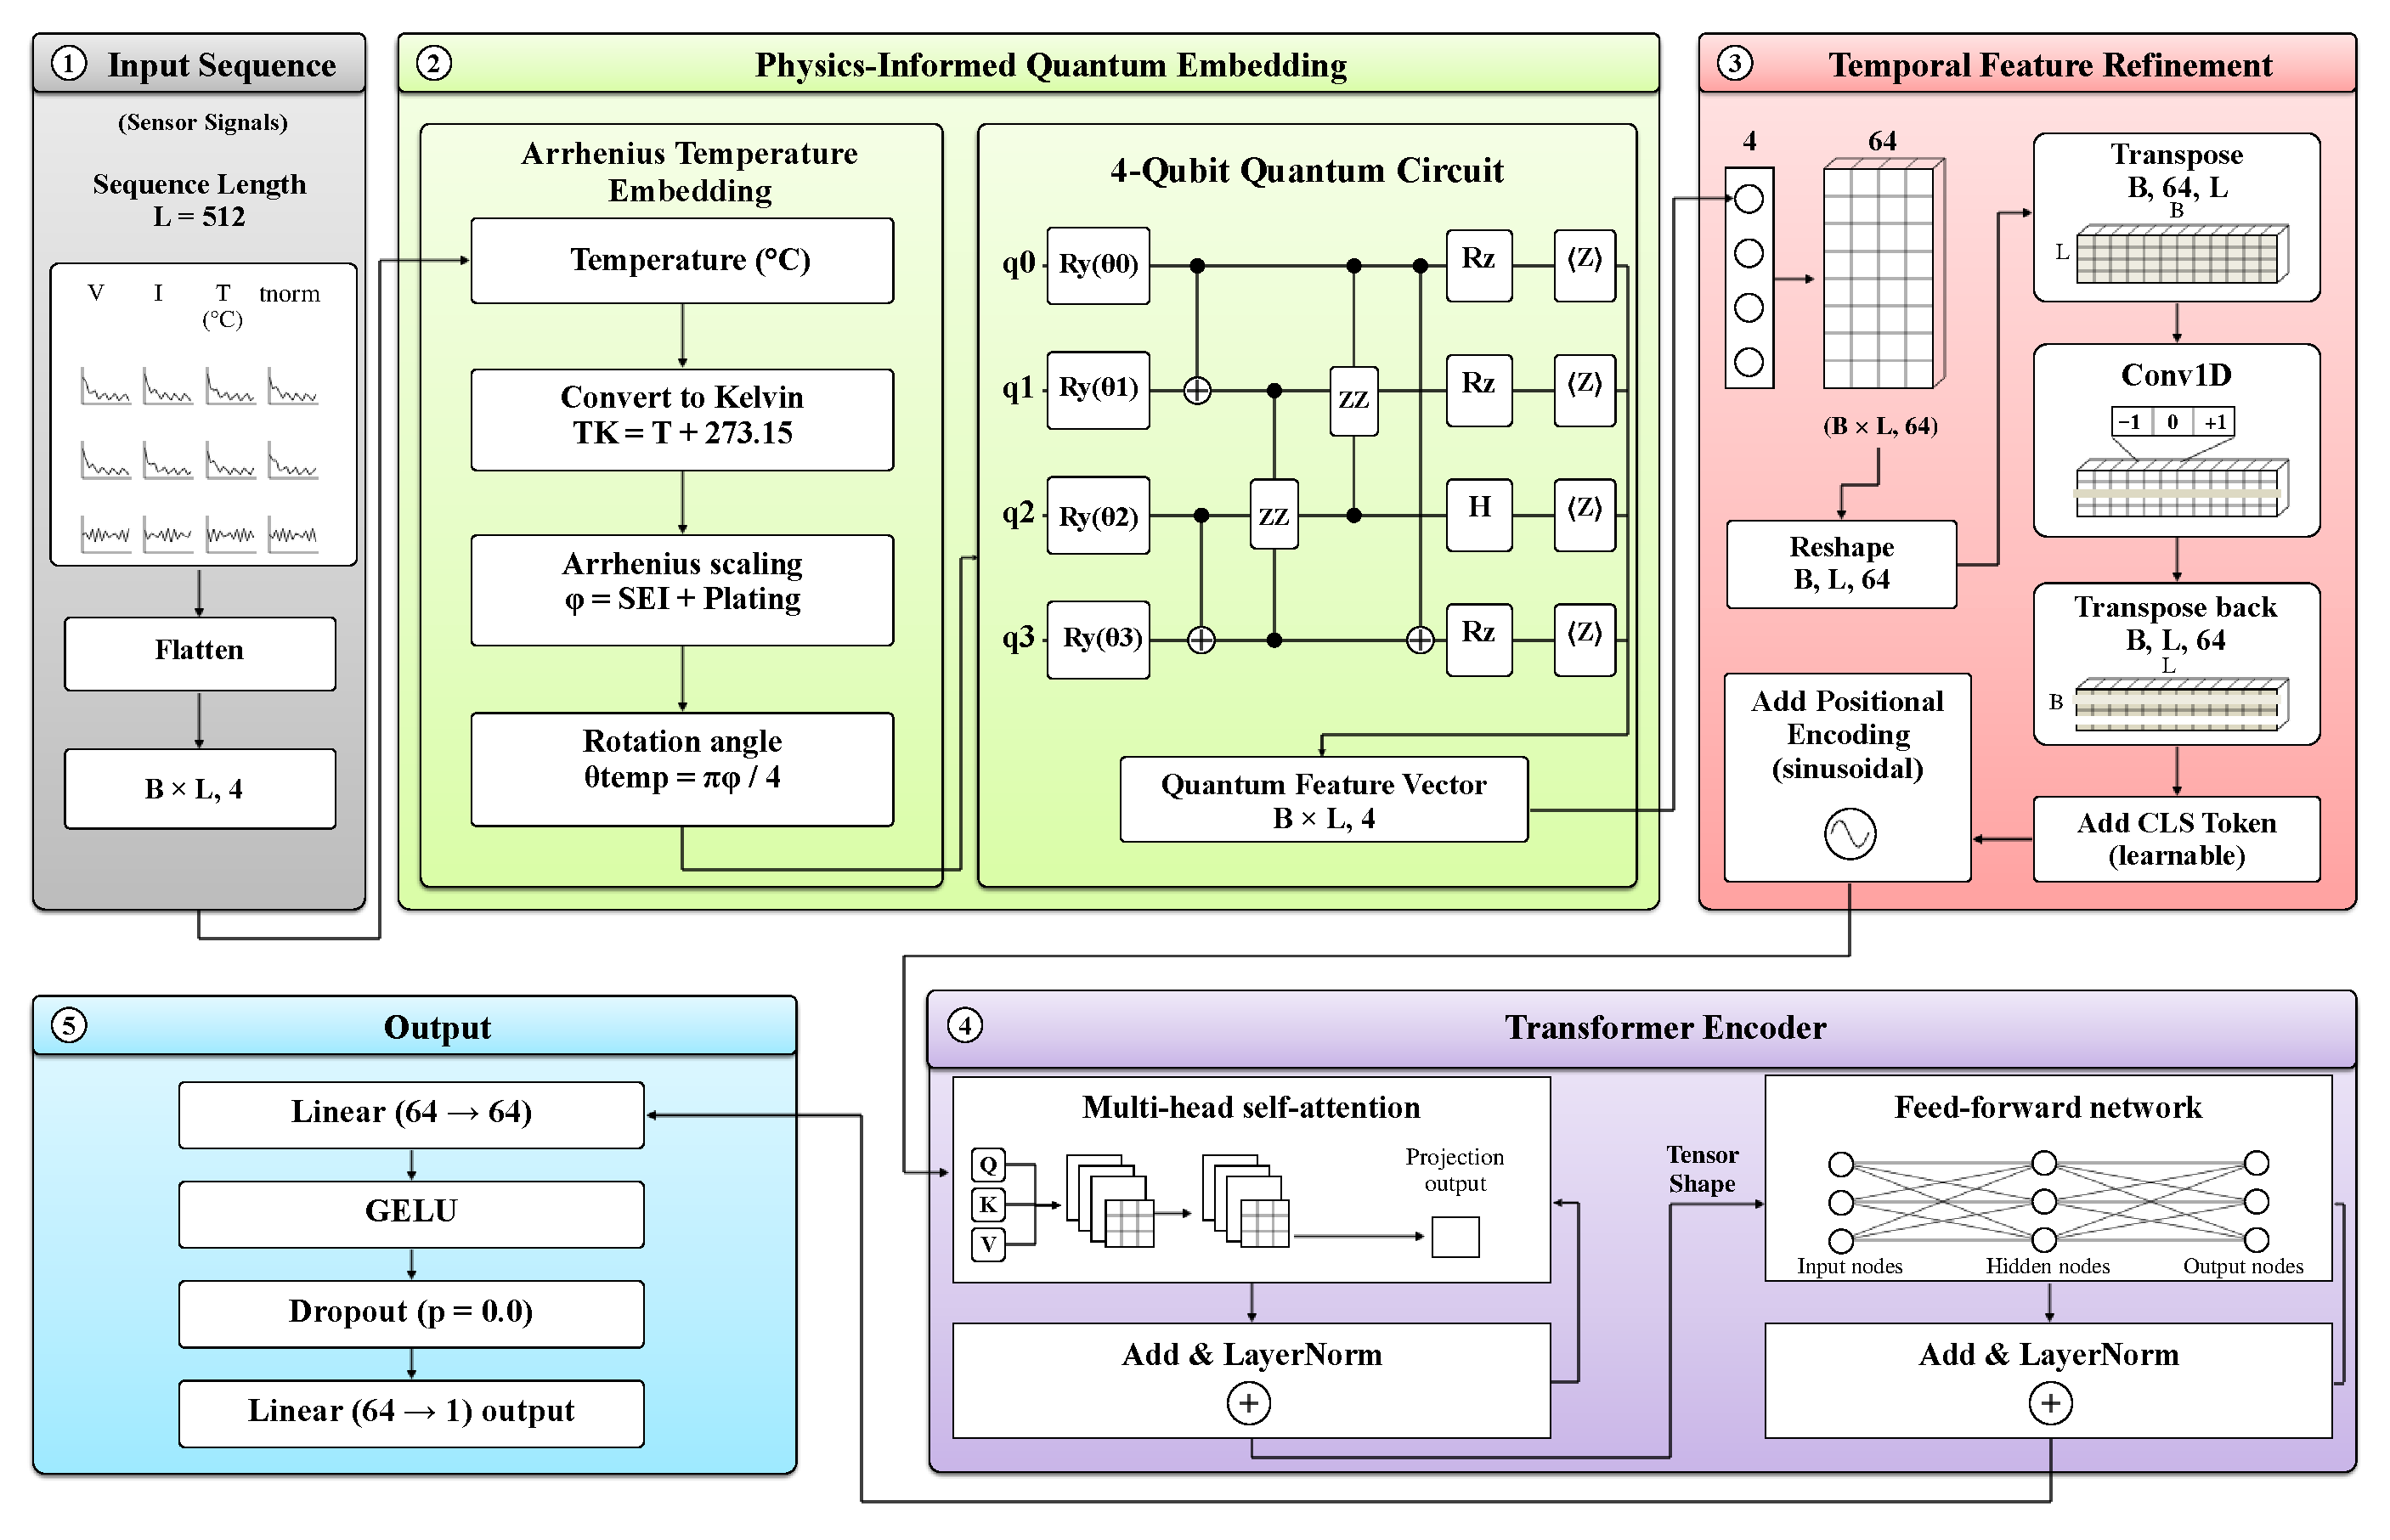
\includegraphics[width=\linewidth]{figs/TE-Q-Architecture-Final.pdf}
  \caption{Overall five-stage architecture of TE-Q-Transformer: (1)~input sensor sequence ($V, I, T, t_{\mathrm{norm}}$) with sequence length $L = 512$, (2)~physics-guided quantum feature mapping via Arrhenius temperature encoding and a four-qubit parameterized quantum circuit, (3)~temporal feature extraction via Conv1D, (4)~Transformer encoder with learnable $\mathrm{[CLS]}$ token and sinusoidal positional encoding, and (5)~regression output head for SOH estimation.}\label{fig:teq_arch}\label{fig2}
\end{figure}

Figure~\ref{fig:teq_arch} summarizes the operational workflow of TE-Q-Transformer across five stages:

\begin{enumerate}[leftmargin=*,noitemsep,topsep=3pt]
\item \textbf{Input processing:} A multi-channel discharge sequence of dimension $(B, L, 4)$ is assembled from sensor measurements resampled to length $L = 512$. Voltage, current, and normalized time are min--max scaled, while cell temperature remains in degrees Celsius.
\item \textbf{Physics-guided quantum mapping:} At each time step, cell temperature is converted to Kelvin and evaluated through the Arrhenius kinetic terms to yield angle $\theta_T$. Linearly scaled voltage, current, and normalized time provide angles $\theta_V, \theta_I, \theta_t$. The four angles are encoded into a four-qubit register, entangled via $U_{\mathrm{rich}}$, and measured under Pauli-$Z$ observables to produce a bounded feature vector $\mathbf{q} \in [-1, 1]^4$.
\item \textbf{Latent projection and local convolution:} The quantum output is projected to $d_{\mathrm{model}} = 64$ by a linear adapter. A one-dimensional convolution over the temporal dimension extracts local sequence patterns.
\item \textbf{Global self-attention:} A learnable $\mathrm{[CLS]}$ token is prepended to the sequence, and sinusoidal positional encodings are added. The three-layer Transformer encoder applies multi-head self-attention across the full sequence of $513$ tokens, allowing the $\mathrm{[CLS]}$ token to aggregate sequence context.
\item \textbf{SOH prediction:} The encoded representation of the $\mathrm{[CLS]}$ token is passed to a two-layer MLP regression head to yield the final scalar SOH prediction $\hat{y}$.
\end{enumerate}

The experimental protocol, baseline comparisons, and empirical performance of this framework are evaluated in Section~\ref{sec:experiments}.







\section{Experimental Results}\label{sec:experiments}

This section evaluates TE-Q-Transformer on the NASA and CALCE battery datasets and compares it with ten baseline architectures. Ablation and reproducibility studies are then presented.

\subsection{Experiment}\label{sec:experiment}

\subsubsection{Experimental Protocol}\label{sec:experimental_protocol}

Each discharge cycle is represented as a multi-channel sequence of fixed length $L = 512$. The measurements are resampled by linear interpolation over the discharge interval. The four input channels are terminal voltage $V$, load current $I$, cell surface temperature $T_C$, and normalized intra-cycle time $t_{\mathrm{norm}}$.

During discharge, the load current follows a negative sign convention. The current is $-2.0\,\mathrm{A}$ for the $24\,^\circ\mathrm{C}$ and $4\,^\circ\mathrm{C}$ cells and $-4.0\,\mathrm{A}$ for the $43\,^\circ\mathrm{C}$ cells. Temperature values correspond to the constant ambient setpoint of each cell: $24\,^\circ\mathrm{C}$, $43\,^\circ\mathrm{C}$, or $4\,^\circ\mathrm{C}$.

Feature scaling uses min--max normalization fitted exclusively on the 660 training cycles for voltage, current, and normalized time. The fitted training bounds are $[1.7616\,\mathrm{V}, 4.2333\,\mathrm{V}]$ for voltage, $[-4.0303\,\mathrm{A}, 0.0072\,\mathrm{A}]$ for current, and $[0.0, 1.0]$ for normalized time. The scaled channels are clipped to $[0.0, 1.0]$ before quantum encoding. Cell temperature is retained in degrees Celsius at the model input and converted to Kelvin before the Arrhenius computation. Data partitioning was completed before sequence interpolation and normalization, and the scaling parameters were fitted only on the training data. No test-guided hyperparameter tuning, model selection, or post-hoc calibration was used.

Performance is evaluated using five metrics: RMSE, MAE, MAPE, $R^2$, and MaxE. Their definitions are given below.
\begin{align}
\mathrm{RMSE} &= \sqrt{\frac{1}{N}\sum_{i=1}^{N}(y_i-\hat{y}_i)^2}, \label{eq:rmse} \\
\mathrm{MAE} &= \frac{1}{N}\sum_{i=1}^{N}|y_i-\hat{y}_i|, \label{eq:mae} \\
\mathrm{MAPE} &= \frac{1}{N}\sum_{i=1}^{N}\left|\frac{y_i-\hat{y}_i}{y_i}\right|\times 100\%, \label{eq:mape} \\
R^2 &= 1-\frac{\sum_{i=1}^{N}(y_i-\hat{y}_i)^2}{\sum_{i=1}^{N}(y_i-\bar{y})^2}, \label{eq:r2} \\
\mathrm{MaxE} &= \max_{1\le i\le N}|y_i-\hat{y}_i|. \label{eq:maxe}
\end{align}
Here, $y_i$ is the reference SOH defined in Eq.~\eqref{eq:soh_def}, $\hat{y}_i$ is the predicted SOH, $\bar{y}$ is the mean reference SOH, and $N$ is the number of evaluated cycles. For the NASA benchmark, RMSE, MAE, MAPE, and $R^2$ are computed as the unweighted arithmetic mean across B0018, B0032, and B0053-test. MaxE is the maximum absolute error across all evaluated test cycles.

\subsubsection{Implementation Details}\label{sec:implementation_details}

All models were implemented in PyTorch and run in a Kaggle Notebook environment with two NVIDIA Tesla T4 GPUs, each providing 15.84\,GB of VRAM. The computations were assigned to a single GPU, \texttt{cuda:0}. Multi-GPU wrappers such as \texttt{DataParallel} and \texttt{DistributedDataParallel} were not used. The software environment used Python 3.10, PyTorch 2.1.0+cu128, CUDA 12.8, and PennyLane 0.41.1. All training and inference used float32 precision without automatic mixed precision.

The quantum circuits were simulated on the CPU using the PennyLane \texttt{default.qubit} state-vector backend. Gradients were computed through PyTorch autograd with \texttt{diff\_method="backprop"}. Random seeds were fixed in Python, NumPy, and PyTorch for all runs. cuDNN deterministic mode was enabled and benchmark mode was disabled.

All models were trained with mean squared error loss using the AdamW optimizer, an initial learning rate of $10^{-3}$, and a maximum of 80 epochs. Gradient norms were clipped to a maximum $L_2$ norm of 1.0. The learning rate was reduced using \texttt{ReduceLROnPlateau} with a reduction factor of 0.5, a patience of 10 epochs, and a minimum learning rate of $10^{-6}$. The scheduler monitored the training loss. Early stopping used a patience of 20 epochs based on training loss. No independent validation split was used. Checkpoints were selected based on the lowest training MSE across completed epochs. The batch size was 8 for TE-Q-Transformer and the eight classical baseline models and 16 for QLSTM and QNN-GRU.

Three training campaigns were used in this study. The reference TE-Q-Transformer run used for the primary NASA benchmark in Table~\ref{tab:teq_nasa_reference} and zero-shot CALCE transfer in Table~\ref{tab:calce} was trained with a weight decay of $5\times 10^{-2}$ and random seed 42. It reached its lowest training loss of $1.183\times 10^{-4}$ at epoch 80.

The independent retraining campaign in Section~\ref{sec:study_reproducibility} used a weight decay of $1\times 10^{-2}$ and seed 42. The best checkpoint occurred at epoch 76 with a training loss of $1.270\times 10^{-4}$ and a macro RMSE of $0.0239$.

The multi-seed study used five predefined random seeds from 42 to 46 with a weight decay of $1\times 10^{-2}$. The ten baseline models used a weight decay of $1\times 10^{-2}$ and seed 42. Controlled ablation runs in Section~\ref{sec:ablation} used the reference weight decay of $5\times 10^{-2}$ and seed 42.

\subsubsection{Baseline and Comparison Methods}\label{sec:baseline_comparison}

Ten baseline models from three methodological categories were selected for comparison with TE-Q-Transformer:

\paragraph{Recurrent and convolutional models}
\begin{itemize}[leftmargin=*,noitemsep,topsep=2pt]
\item Hochreiter's LSTM~\citep{hochreiter1997}: a recurrent neural network that regulates sequential information flow using dedicated memory cells with input, forget, and output gates.
\item Cho's GRU~\citep{cho2014}: a gated recurrent architecture that captures sequence dynamics using reset and update gates without separate memory cells.
\item Wang's CNN1D~\citep{wang2017time}: a one-dimensional convolutional neural network that extracts local temporal features directly from multi-channel input sequences.
\item Bai's TCN~\citep{bai2018empirical}: a temporal convolutional network that models sequential dependencies across extended receptive fields using causal dilated convolutions.
\end{itemize}

\paragraph{Long-sequence and transformer models}
\begin{itemize}[leftmargin=*,noitemsep,topsep=2pt]
\item Zeng's DLinear~\citep{zeng2023}: a linear temporal model that maps sequences through moving-average trend-seasonal decomposition and single-layer projections.
\item Vaswani's Transformer~\citep{vaswani2017}: an encoder architecture that models sequence relationships using multi-head self-attention.
\item Nie's PatchTST~\citep{nie2023patchtst}: a transformer framework that segments multivariate series into sub-series patches while processing individual channels independently.
\item Liu's iTransformer~\citep{liu2024itransformer}: an inverted transformer architecture that embeds entire variates as tokens and applies self-attention across variate representations.
\end{itemize}

\paragraph{Quantum and hybrid models}
\begin{itemize}[leftmargin=*,noitemsep,topsep=2pt]
\item Wang's QLSTM~\citep{wang2026prediction}: a hybrid recurrent architecture that combines a 4-qubit parameterized quantum circuit with an LSTM sequence model.
\item Soon's QNN-GRU~\citep{soon2025hybrid}: a hybrid architecture that combines a 4-qubit parameterized quantum neural network with a gated recurrent unit.
\end{itemize}

All baseline models use the same two-layer MLP prediction head with GELU activation, except DLinear, which directly projects the decomposed components. The parameter counts range from $1\,031$ for DLinear to $137\,473$ for iTransformer, as reported in Table~\ref{tab:main_benchmark}.


\subsection{Case Study on the NASA Battery Dataset}\label{sec:nasa_case}

\subsubsection{Dataset Description}\label{sec:nasa_description}

The NASA Ames Prognostics Center of Excellence battery dataset~\citep{saha2007battery} provides the primary case study for evaluating TE-Q-Transformer. The dataset contains run-to-failure cycling records of commercial 18650 cylindrical lithium-ion cells tested in environmental chambers under controlled thermal conditions. Nine cells across three ambient temperatures are included in this study. Cells B0005, B0006, B0007, and B0018 were operated at a nominal room temperature of $24\,^\circ\mathrm{C}$. Cells B0029, B0030, B0031, and B0032 were cycled at an elevated temperature of $43\,^\circ\mathrm{C}$. Cell B0053 was cycled at a low temperature of $4\,^\circ\mathrm{C}$. Together, these nine cells contribute 847 discharge cycles. Electrochemical impedance spectroscopy measurements present in the raw records are omitted from this study.

Figure~\ref{fig:nasa_setup} illustrates the experimental testbed and the cycling workflow. Representative discharge measurements appear in Figure~\ref{fig:nasa_signal_overview}. Discharge voltage curves exhibit lower plateaus and earlier cutoff times as cells degrade, shown in Figure~\ref{fig:nasa_signal_overview}a--c. Galvanostatic discharge currents follow a negative sign convention in Figure~\ref{fig:nasa_signal_overview}d, while cell surface temperatures track their chamber setpoints during cycling in Figure~\ref{fig:nasa_signal_overview}e. Over repeated cycling, discharge capacity declines gradually with localized recovery following rest periods, as illustrated in Figure~\ref{fig:nasa_signal_overview}f.

\begin{figure}[t]
\centering
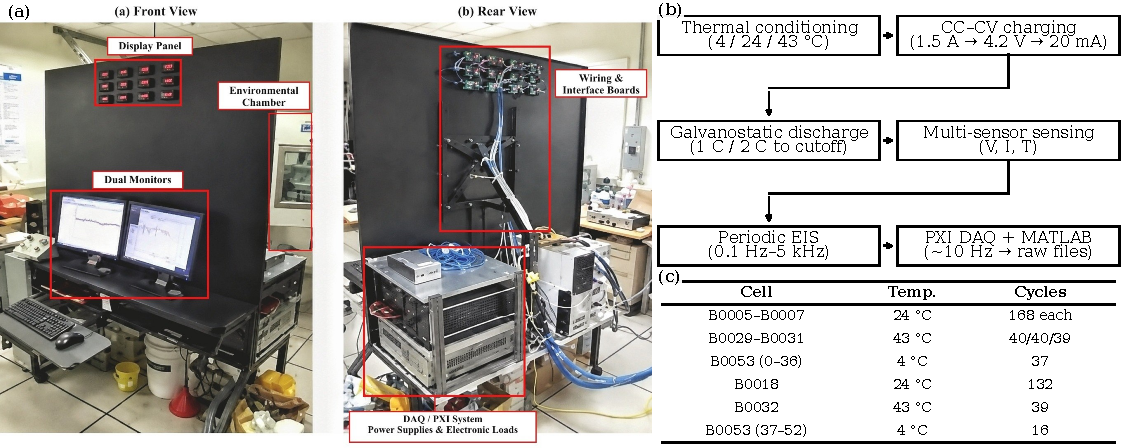
\includegraphics[width=0.82\textwidth]{figs/fig2_nasa_experimental_setup.pdf}
\caption{NASA lithium-ion battery experimental platform and cycling protocol: (a)~battery testbed with environmental chamber (adapted from Figure~7 in Saha and Goebel~\cite{saha2009modeling}), (b)~cycling and measurement workflow, and (c)~evaluated 18650 cells across the three operating temperature regimes.}\label{fig:nasa_setup}
\end{figure}

\begin{figure}[t]
\centering
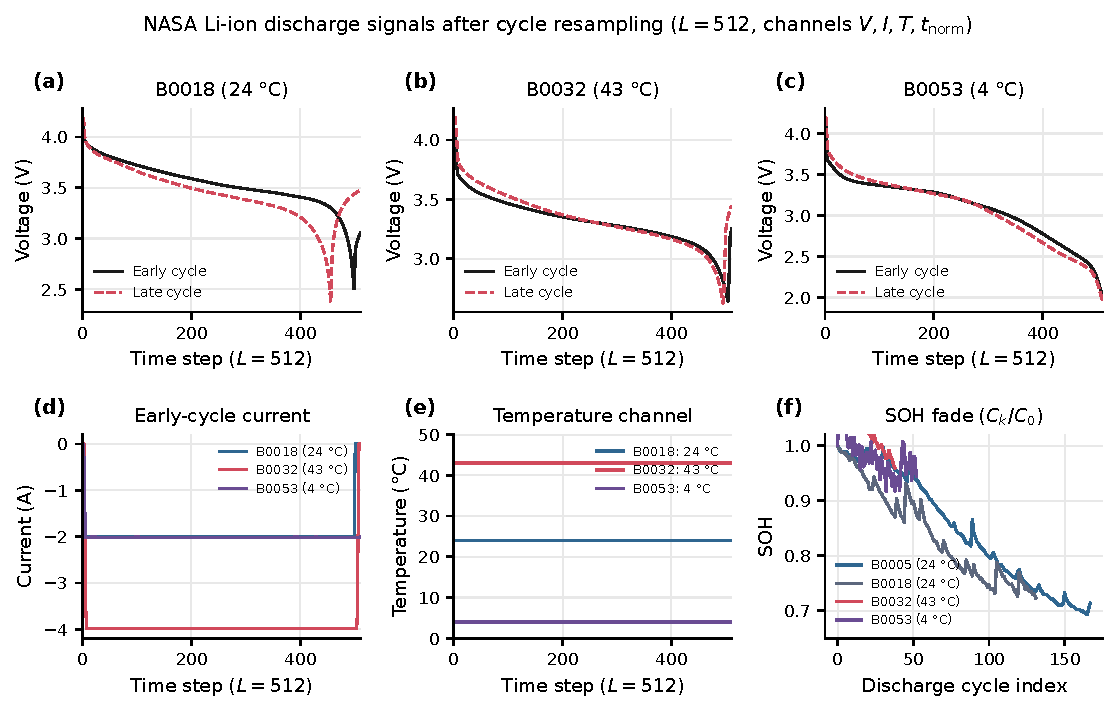
\includegraphics[width=0.82\textwidth]{figs/fig_nasa_signal_overview.pdf}
\caption{Representative discharge measurements and capacity degradation from the NASA battery dataset ($L = 512$): (a)--(c)~discharge voltage profiles for early and late cycles across cells B0018 ($24\,^\circ\mathrm{C}$), B0032 ($43\,^\circ\mathrm{C}$), and B0053 ($4\,^\circ\mathrm{C}$); (d)~load current profiles ($-2.0\,\mathrm{A}$ and $-4.0\,\mathrm{A}$); (e)~battery surface temperatures; and (f)~SOH trajectories ($C_k / C_0$) showing capacity fade and localized recovery.}\label{fig:nasa_signal_overview}
\end{figure}

To quantify capacity degradation across cycles, the state of health is evaluated as defined in Eq.~\eqref{eq:soh_def}, representing the ratio of delivered discharge capacity $C_k$ to initial capacity $C_0$.

\subsubsection{Experimental Setup}\label{sec:nasa_setup}

The evaluation on the NASA dataset assesses cross-cell transfer and temporal extrapolation. Cells B0018 and B0032 are withheld entirely from training as unseen test cells. In contrast, for cell B0053, early cycles 0--36 are included in training, whereas cycles 37--52 are withheld as a temporal holdout. Table~\ref{tab:exp_split} details this data allocation.

\begin{table}[t]
\centering
\small
\caption{NASA experimental setup and evaluation scenarios.}\label{tab:exp_split}
\begin{tabular}{@{}llcll@{}}
\toprule
Cell(s) & Temperature & Cycles & Partition & Evaluation scenario \\
\midrule
B0005, B0006, B0007 & $24\,^\circ\mathrm{C}$ & 168, 167, 168 (503 total) & Train & Seen cells \\
B0029, B0030, B0031 & $43\,^\circ\mathrm{C}$ & 40, 40, 40 (120 total) & Train & Seen cells \\
B0053 (cycles 0--36) & $4\,^\circ\mathrm{C}$ & 37 & Train & Early segment only \\
B0018 & $24\,^\circ\mathrm{C}$ & 132 & Test & Unseen-cell evaluation \\
B0032 & $43\,^\circ\mathrm{C}$ & 39 & Test & Unseen-cell evaluation \\
B0053 (cycles 37--52) & $4\,^\circ\mathrm{C}$ & 16 & Test & Temporal holdout \\
\bottomrule
\end{tabular}
\end{table}

This benchmark includes 660 training cycles across seven cells and 187 test cycles across the three evaluation settings. Because early cycles of B0053 are in the training set, this test assesses temporal progression on a partially observed cell rather than transfer to an unseen cell. In addition, all three operating temperatures appear in the training pool. The NASA evaluation therefore assesses cross-cell transfer and temporal extrapolation under known thermal conditions, rather than generalization to unseen temperatures.

\subsubsection{Results and Analysis}\label{sec:nasa_results}

Table~\ref{tab:teq_nasa_reference} reports the performance of the reference TE-Q-Transformer across the three NASA test settings. Across all three settings, the model achieves a macro RMSE of $0.0168$ and a macro $R^2$ of $0.870$. Estimation accuracy varies across the individual operating regimes. Unseen cell B0018, evaluated at $24\,^\circ\mathrm{C}$, exhibits the highest error among the test cases, yielding an RMSE of $0.0271$. Unseen cell B0032 at $43\,^\circ\mathrm{C}$ and the temporal holdout B0053 at $4\,^\circ\mathrm{C}$ show lower errors, recording RMSE values of $0.0119$ and $0.0113$, respectively.

Figure~\ref{fig:nasa_reference_trajectories} illustrates the predicted SOH trajectories and the pooled parity analysis. On cell B0018, shown in Figure~\ref{fig:nasa_reference_trajectories}a, the predicted trajectory tracks the overall fade pattern but deviates from the experimental curve in later cycles, giving the maximum absolute error of $0.1022$ in the benchmark. On cells B0032 and B0053, shown in Figure~\ref{fig:nasa_reference_trajectories}b and c, predictions closely match the true degradation profiles throughout cycling. In the pooled parity comparison in Figure~\ref{fig:nasa_reference_trajectories}d, the predictions across all 187 test cycles align closely with the ideal diagonal.

\begin{figure}[t]
\centering
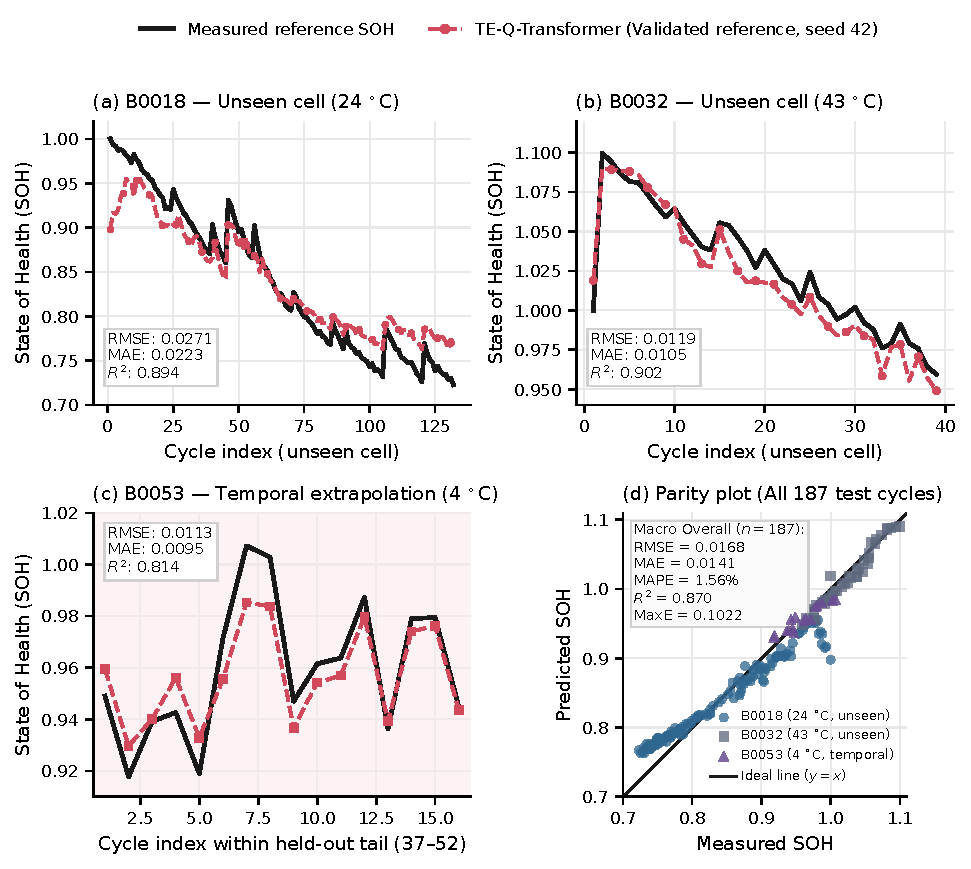
\includegraphics[width=0.82\textwidth]{figs/fig_nasa_reference_trajectories.pdf}
\caption{SOH prediction trajectories and pooled parity analysis for the reference TE-Q-Transformer on the NASA test settings: (a)~unseen cell B0018 at $24\,^\circ\mathrm{C}$; (b)~unseen cell B0032 at $43\,^\circ\mathrm{C}$; (c)~temporal extrapolation on B0053 over cycles 37--52 at $4\,^\circ\mathrm{C}$; and (d)~pooled measured versus predicted SOH across all 187 test cycles.}\label{fig:nasa_reference_trajectories}
\end{figure}

\begin{table}[t]
\centering
\small
\caption{Reference TE-Q-Transformer performance on the three NASA test settings.}\label{tab:teq_nasa_reference}
\begin{tabular}{@{}lccccc@{}}
\toprule
Setting & RMSE & MAE & MAPE (\%) & $R^2$ & MaxE \\
\midrule
B0018 (unseen, $24\,^\circ\mathrm{C}$) & 0.0271 & 0.0223 & 2.66 & 0.894 & 0.1022 \\
B0032 (unseen, $43\,^\circ\mathrm{C}$) & 0.0119 & 0.0105 & 1.03 & 0.902 & 0.0237 \\
B0053-test (temporal, $4\,^\circ\mathrm{C}$) & 0.0113 & 0.0095 & 0.99 & 0.814 & 0.0220 \\
\midrule
Macro & 0.0168 & 0.0141 & 1.56 & 0.870 & 0.1022 \\
\bottomrule
\end{tabular}
\par\vspace{2pt}\raggedright\footnotesize\textit{Note:} RMSE, MAE, MAPE, and $R^2$ in the macro row are unweighted arithmetic means across the three test settings, whereas MaxE is the maximum absolute error across all 187 test cycles.
\end{table}

\subsection{External Validation on the CALCE Battery Dataset}\label{sec:calce}

To determine whether the NASA-trained model transfers across distinct battery platforms without retraining, an external validation was conducted on the CALCE dataset.

\subsubsection{Dataset Description}\label{sec:calce_description}

This evaluation uses cycling records from four CS2 cells from the Center for Advanced Life Cycle Engineering at the University of Maryland~\citep{w9rg-7173-25}: CS2\_35, CS2\_36, CS2\_37, and CS2\_38. These prismatic lithium cobalt oxide cells, with chemical composition $\mathrm{LiCoO}_2$ and a nominal capacity of $1.1$\,Ah, differ from the cylindrical NASA cells in cell format, chemistry, and cycling profile. Cycling consisted of constant-current constant-voltage charging at $0.5\mathrm{C}$ to $4.2$\,V and galvanostatic $1\mathrm{C}$ discharge to a cutoff voltage of $2.7$\,V.

Discharge cycles were screened with physical criteria to ensure consistent cycling conditions. An accepted discharge cycle required a mean current below $-0.4\,\mathrm{A}$, an initial voltage of at least $3.6\,\mathrm{V}$, a terminal cutoff voltage of at most $3.2\,\mathrm{V}$, and a delivered capacity between $0.15$\,Ah and $1.30$\,Ah. In addition, test time was required to increase monotonically across at least 16 raw measurement points. The screening retained $3\,909$ discharge cycles across the four cells. The retained cycles were resampled by linear interpolation to a uniform length of $L = 512$ points. Because the published CALCE logs do not record continuous thermocouple data, the temperature input was assigned a constant ambient value of $23\,^\circ\mathrm{C}$.

\subsubsection{Cross-Dataset Validation Setup}\label{sec:calce_setup}

The evaluation applies a zero-shot cross-dataset protocol to test whether the learned model generalizes across battery platforms without fine-tuning. The NASA-trained TE-Q-Transformer and the corresponding NASA-fitted feature scaler are applied without modification. No CALCE data are used for model training, validation, hyperparameter tuning, or calibration. Voltage, current, and normalized time are scaled using the min--max parameters fitted on the NASA training split, while temperature is fixed at $23\,^\circ\mathrm{C}$. All four CS2 cells serve as external unseen test cells. Because the temperature channel is held constant, this experiment evaluates transfer across battery chemistry, cell format, and cycling conditions rather than temperature generalization.

\subsubsection{Results and Analysis}\label{sec:calce_results}

Table~\ref{tab:calce} reports the performance of the frozen NASA-trained model across all $3\,909$ accepted CALCE discharge cycles, alongside a baseline predicting a constant SOH of $1.0$.

\begin{table}[t]
\centering
\small
\caption{Zero-shot NASA$\rightarrow$CALCE performance of the NASA-trained TE-Q-Transformer, with a constant predictor reference. Pooled metrics concatenate all $3\,909$ accepted discharge windows. Mean bias is predicted SOH minus true SOH.}\label{tab:calce}
\begin{tabular}{@{}lcccccc@{}}
\toprule
Cell & RMSE & MAE & MAPE (\%) & $R^2$ & MaxE & Mean bias \\
\midrule
CS2\_35 & 0.2933 & 0.2415 & 42.56 & $-$2.070 & 0.8029 & $+$0.2415 \\
CS2\_36 & 0.3731 & 0.2937 & 77.27 & $-$1.567 & 0.8380 & $+$0.2937 \\
CS2\_37 & 0.3483 & 0.2803 & 65.73 & $-$1.776 & 0.8284 & $+$0.2803 \\
CS2\_38 & 0.3061 & 0.2524 & 45.93 & $-$2.115 & 0.8344 & $+$0.2524 \\
\midrule
Pooled (TE-Q) & 0.3325 & 0.2676 & 58.18 & $-$1.789 & 0.8380 & $+$0.2676 \\
Constant SOH $=1.0$ (pooled) & 0.3277 & 0.2602 & 57.21 & $-$1.708 & 0.8595 & $+$0.2602 \\
\bottomrule
\end{tabular}
\end{table}

On the pooled test cycles, TE-Q-Transformer yields an RMSE of $0.3325$ and an $R^2$ of $-1.789$. This performance is comparable to the constant reference prediction, which achieves a pooled RMSE of $0.3277$ and an $R^2$ of $-1.708$. Across individual cells, RMSE remains between $0.2933$ and $0.3731$, with negative $R^2$ values throughout.

The transferred predictions show a restricted range and positive residual bias. Measured SOH spans approximately $0.14$--$1.00$ across the pooled CALCE cycles, whereas the predictions remain confined to $0.978$--$1.041$, spanning only $7.4\%$ of the true degradation range. Because predictions remain close to $1.0$, residuals are positive for all cycles and increase as the cells degrade.

These results show that representations learned on the NASA benchmark do not transfer directly to the CALCE platform in a zero-shot setting. Several domain differences between the two datasets may contribute to this behavior. NASA cells are cylindrical units with nickel-cobalt-aluminum chemistry discharged at $2.0\,\mathrm{A}$ or $4.0\,\mathrm{A}$, whereas CALCE cells are prismatic units with lithium cobalt oxide chemistry discharged at a $1\mathrm{C}$ rate of $1.1\,\mathrm{A}$. The constant $23\,^\circ\mathrm{C}$ input does not represent the thermal variation present in the NASA measurements.

\subsection{Comparison with Baseline Methods}\label{sec:comparison_baselines}

Table~\ref{tab:main_benchmark} compares TE-Q-Transformer with the ten baseline models across the three methodological categories on the NASA benchmark.

\begin{table}[t]
\centering
\small
\caption{NASA performance comparison under the fixed NASA benchmark. Overall metrics are unweighted arithmetic means across B0018, B0032, and B0053-test. TE-Q-Transformer is the reference configuration.}\label{tab:main_benchmark}
\begin{tabular}{@{}lcccccc@{}}
\toprule
Model & RMSE & MAE & MAPE (\%) & $R^2$ & MaxE & Params \\
\midrule
\multicolumn{7}{@{}l}{\textit{Recurrent and convolutional models}} \\
LSTM & 0.0416 & 0.0367 & 4.07 & $-$0.076 & 0.0904 & 71\,105 \\
GRU & 0.0642 & 0.0565 & 6.22 & $-$1.680 & 0.1631 & 54\,465 \\
CNN1D & 0.0509 & 0.0457 & 4.78 & $-$3.191 & 0.1245 & 47\,041 \\
TCN & 0.0535 & 0.0452 & 5.09 & $-$0.341 & 0.1491 & 91\,841 \\
\midrule
\multicolumn{7}{@{}l}{\textit{Long-sequence and transformer models}} \\
DLinear & 0.0624 & 0.0568 & 5.88 & $-$2.232 & 0.1853 & 1\,031 \\
Transformer & 0.0346 & 0.0287 & 3.14 & 0.218 & 0.1123 & 80\,257 \\
PatchTST & 0.0387 & 0.0333 & 3.69 & 0.321 & 0.1457 & 109\,962 \\
iTransformer & 0.0341 & 0.0298 & 3.28 & 0.533 & 0.1165 & 137\,473 \\
\midrule
\multicolumn{7}{@{}l}{\textit{Quantum and hybrid models}} \\
QLSTM & 0.0445 & 0.0386 & 4.35 & $-$0.336 & 0.1066 & 37\,853 \\
QNN-GRU & 0.0304 & 0.0248 & 2.61 & 0.258 & \textbf{0.0725} & 29\,533 \\
\midrule
\textbf{TE-Q-Transformer (Proposed)} & \textbf{0.0168} & \textbf{0.0141} & \textbf{1.56} & \textbf{0.870} & 0.1022 & 92\,554 \\
\bottomrule
\end{tabular}
\end{table}

The recurrent baselines, LSTM and GRU, record large macro errors on the benchmark, yielding macro RMSE values of $0.0416$ and $0.0642$, with negative $R^2$ scores of $-0.076$ and $-1.680$. The convolutional architectures, CNN1D and TCN, similarly yield negative macro $R^2$ values of $-3.191$ and $-0.341$, with maximum errors exceeding $0.12$. Although CNN1D achieves an RMSE of $0.0255$ on unseen cell B0018, higher errors on the other test cells result in a higher macro RMSE across the benchmark.

The attention-based architectures, Transformer, PatchTST, and iTransformer, show lower macro errors than the recurrent and convolutional baselines, yielding macro RMSE values between $0.0341$ and $0.0387$ and positive $R^2$ scores from $0.218$ to $0.533$. Among the attention-based models, iTransformer records the lowest macro RMSE and highest $R^2$. In contrast, the linear decomposition baseline, DLinear, records a macro RMSE of $0.0624$ and an $R^2$ of $-2.232$. Across all models in this category, maximum errors exceed $0.11$.

The two hybrid quantum-recurrent baselines show differing performance on the benchmark. QNN-GRU obtains a macro RMSE of $0.0304$, an $R^2$ of $0.258$, and the lowest maximum error among the models in Table~\ref{tab:main_benchmark} at $0.0725$. Conversely, QLSTM records a macro RMSE of $0.0445$ and an $R^2$ of $-0.336$, with an RMSE close to that of the classical LSTM.

TE-Q-Transformer records the lowest macro RMSE and highest macro $R^2$ across the benchmark, achieving values of $0.0168$ and $0.870$, respectively. QNN-GRU, however, yields a lower maximum absolute error of $0.0725$, compared with $0.1022$ for TE-Q-Transformer. Because the quantum layers are executed on a classical simulator via PennyLane \texttt{default.qubit}, this design incurs simulation overhead, and no physical hardware acceleration is claimed.

\subsection{Further Study}\label{sec:ablation}

\subsubsection{Effect of Temperature Representation}\label{sec:study_temp}

To isolate the effect of the physics-guided temperature representation, the Arrhenius-based encoding was evaluated against conventional linear temperature normalization using the same base architecture. Results are presented in Figure~\ref{fig:ablation_combined}a and Table~\ref{tab:physics}.

Replacing linear temperature normalization with the physics-guided encoding reduces the macro RMSE from $0.0201$ to $0.0168$, corresponding to a $16.5\%$ relative reduction in macro RMSE. However, this performance difference is not uniform across individual cells. On unseen cell B0032, RMSE decreases by $34.8\%$, and on the B0053 temporal holdout, RMSE decreases by $40.4\%$. Conversely, on unseen cell B0018, RMSE increases by $17.5\%$. These results indicate that while the physics-guided encoding reduces overall benchmark error, its effect depends on cell-specific degradation behavior and is not uniform across all individual cells.

\subsubsection{Effect of Quantum and Architectural Components}\label{sec:study_components}

To evaluate the structural design choices of TE-Q-Transformer, controlled ablations were conducted for degradation mechanisms, quantum embedding, and architectural components, with results summarized in Figure~\ref{fig:ablation_combined}b--d and Table~\ref{tab:physics}.

Within the degradation-mechanism ablation campaign, combining SEI formation and lithium plating yields the lowest macro RMSE at $0.0215$. The lithium-plating-only configuration records an RMSE of $0.0249$, while the SEI-only configuration records $0.0330$. Both trainable activation-energy parameters were initialized at $3.0$. They converged to learned values of $E_{a,\mathrm{sei}} = 1.981$ and $E_{a,\mathrm{pl}} = 2.820$. These values represent empirical parameters optimized from data rather than measured thermodynamic constants.

To test the predictive contribution of the quantum circuit against a classical nonlinear mapping, the 4-qubit variational circuit was replaced with a near-parameter-matched classical multi-layer perceptron under the same physics-guided encoding and transformer architecture, illustrated in Figure~\ref{fig:ablation_combined}c. The classical model contains $92\,695$ parameters, comparable to the $92\,554$ parameters of the quantum model. Under this controlled comparison, the quantum configuration records a macro RMSE of $0.0215$ and an $R^2$ of $0.610$, whereas the classical counterpart records an RMSE of $0.0431$ and an $R^2$ of $-0.746$. The comparison therefore reflects the tested quantum feature mapping under classical simulation rather than physical quantum hardware performance.

Systematic modification of the architecture shows how individual components affect estimation error, as detailed in Figure~\ref{fig:ablation_combined}d. The largest error increases occur when replacing the rich entangler with a basic entangler, which raises the macro RMSE by $0.0221$ to $0.0388$, and when removing positional encoding, which increases RMSE by $0.0162$. Removing the temporal convolution stage or replacing it with a GRU smoother also elevates error, increasing RMSE by $0.0093$ and $0.0107$, respectively. Moderate error increases occur when replacing the CLS token with mean pooling and when adding a residual skip MLP, while adding a Pauli feature map produces the smallest change, with an RMSE increase of $0.0038$.

\begin{figure}[t]
\centering
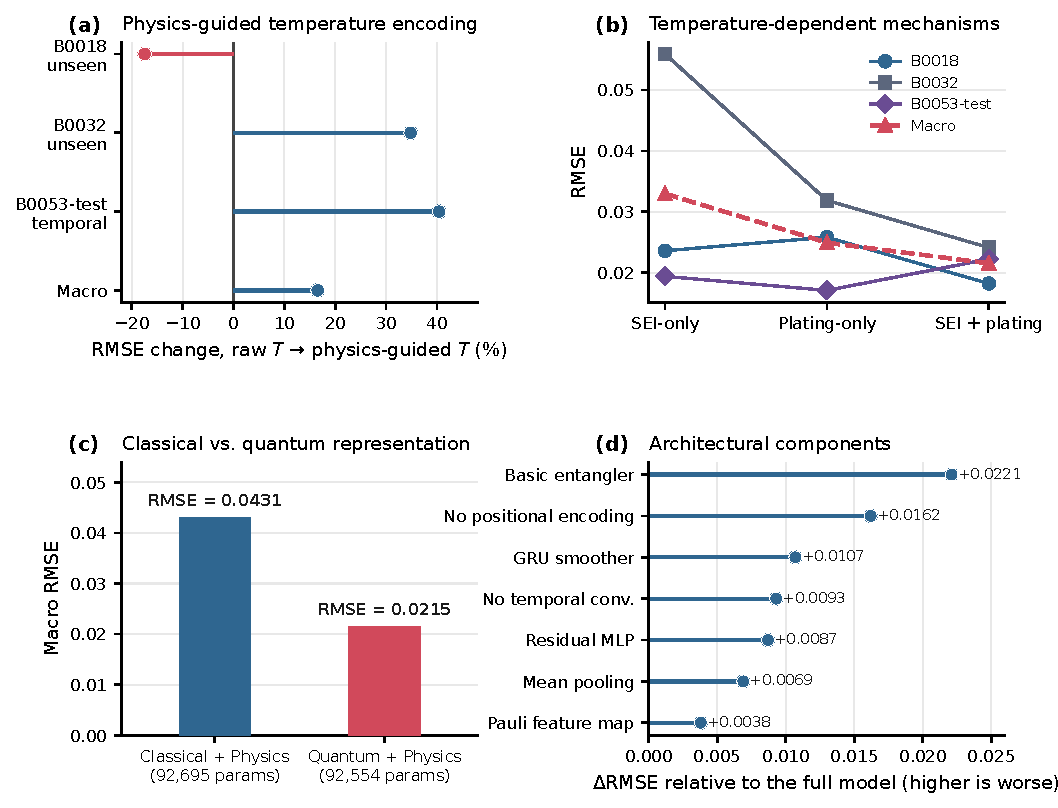
\includegraphics[width=0.82\textwidth]{figs/fig_ablation_combined.pdf}
\caption{Consolidated ablation analysis on the NASA benchmark: (a)~effect of physics-guided temperature encoding on RMSE; (b)~temperature-dependent mechanism ablation (SEI-only, Li-plating-only, and combined); (c)~near-parameter-matched classical versus quantum representation under identical physics-guided encoding; and (d)~architectural component effects as $\Delta\mathrm{RMSE}$ for controlled removals, replacements, and additions.}\label{fig:ablation_combined}
\end{figure}

\begin{table}[t]
\centering
\small\setlength{\tabcolsep}{2.2pt}
\caption{Consolidated ablation results for TE-Q-Transformer on the NASA macro split. Temperature encoding, mechanism, quantum, and architectural variants represent controlled training campaigns.}\label{tab:physics}
\begin{tabular}{@{}llcccc@{}}
\toprule
Campaign & Variant / Modification & RMSE & MAE & MAPE (\%) & $R^2$ \\
\midrule
Temperature representation & Conventional linear normalization & 0.0201 & 0.0171 & 1.84 & 0.723 \\
 & Physics-guided Arrhenius (Reference) & 0.0168 & 0.0141 & 1.56 & 0.870 \\
\midrule
Degradation mechanisms & SEI-only & 0.0330 & 0.0282 & 2.88 & 0.068 \\
 & Li-plating-only & 0.0249 & 0.0208 & 2.21 & 0.592 \\
 & SEI + Li-plating (combined) & 0.0215 & 0.0172 & 1.81 & 0.610 \\
\midrule
Quantum representation & Near-parameter-matched classical MLP ($92\,695$ params) & 0.0431 & 0.0377 & 3.99 & $-$0.746 \\
 & 4-qubit quantum circuit ($92\,554$ params) & 0.0215 & 0.0172 & 1.81 & 0.610 \\
\midrule
Architectural blocks & Basic entangler (replaces rich entangler) & 0.0388 & 0.0320 & 3.53 & 0.342 \\
 & No positional encoding (removes PE) & 0.0330 & 0.0268 & 2.87 & 0.174 \\
 & GRU smoother (replaces temporal conv) & 0.0274 & 0.0217 & 2.38 & 0.649 \\
 & No temporal convolution (removes conv) & 0.0261 & 0.0231 & 2.50 & 0.618 \\
 & Residual MLP (adds skip MLP) & 0.0255 & 0.0214 & 2.29 & 0.545 \\
 & Mean pooling (replaces CLS token) & 0.0237 & 0.0190 & 2.02 & 0.565 \\
 & Pauli feature map (adds Pauli encoding) & 0.0206 & 0.0166 & 1.78 & 0.774 \\
 & Full architecture (Reference) & 0.0168 & 0.0141 & 1.56 & 0.870 \\
\bottomrule
\end{tabular}
\end{table}

\subsubsection{Reproducibility and Run-to-Run Variation}\label{sec:study_reproducibility}

To assess sensitivity to retraining and random initialization, two additional evaluations were conducted. In an independent retraining campaign with weight decay $\lambda = 1\times10^{-2}$, TE-Q-Transformer achieves a macro RMSE of $0.0239$, compared with $0.0168$ for the reference configuration trained with $\lambda = 5\times10^{-2}$.

Across five predefined random seeds from 42 to 46, TE-Q-Transformer records a mean macro RMSE of $0.0244 \pm 0.0096$, MAE of $0.0197 \pm 0.0084$, and an $R^2$ of $0.455 \pm 0.534$. These results show measurable run-to-run variation across random initializations.

\section{Threats to Validity}\label{sec:threats}

\subsection{External Validity}\label{sec:external}
The empirical findings are limited to the NASA PCoE and CALCE laboratory cells used in this study. Within NASA, the training and test cells come from the same laboratory dataset, whereas CALCE provides an external laboratory dataset with different cell format and chemistry. Both datasets comprise small-format laboratory cells cycled under controlled conditions.
% and do not cover pack-level behaviour, field duty cycles, or other open datasets. 
Ambient temperatures on the NASA held-out set span 4\,$^\circ$C, 24\,$^\circ$C, and 43\,$^\circ$C, but those temperatures also appear in training, so the NASA result is a multi-temperature check rather than an unseen-temperature test. CALCE temperature is a constant $23\,^\circ$C fill and is not a temperature-generalization experiment. Performance may therefore change under different chemistries, sampling rates, or vehicle-level data. 
The quantum part of the proposed architecture is also simulated in PennyLane rather than executed on physical quantum hardware.
% so reported gains should be read as evidence for the hybrid classical-simulation pipeline, not as a claim about near-term quantum devices.
In addition, the component ablation in Section~\ref{sec:ablation} was carried out on NASA only; we have not verified that every part of the design contributes in the same way on CALCE, so the CALCE result in Section~\ref{sec:calce} should be read as evidence for the full model rather than for each of its components individually.

\subsection{Internal Validity}\label{sec:internal}
We use a single fixed split combining fully held-out cells with a chronological holdout rather than $k$-fold or leave-one-battery-out rotation. Cells B0018 and B0032 are entirely excluded from training, while B0053 is divided chronologically into early training cycles and a later test segment. This provides cell-level separation for the B0018 and B0032 evaluations, while the B0053 setting evaluates temporal extrapolation on a partially observed cell. Consequently, cold-temperature behavior is not completely unseen. The completed training runs did not use an independent validation split. The CALCE evaluation is zero-shot: no CS2 cell is used for training, scaler fitting, or model selection.
% All models share the same 512-step windows, train-only min-max scaling for voltage, current, and time, and raw Celsius temperature for the Arrhenius gate. 
% This equalizes the protocol, yet hyperparameter choices, training schedules, and our re-implementations of GRU, LSTM, Transformer, QNN-GRU, and QLSTM may still differ from the original papers that motivated those baselines. Residual differences in optimization or capacity could therefore contribute to the observed gaps alongside the proposed architecture.

\subsection{Construct Validity}\label{sec:construct}
SOH is defined as current measured capacity divided by each cell's first-cycle capacity. This is a standard laboratory construct. However, it does not capture impedance growth, power fade, or pack-level state of health used in some BMS settings. 
% The Arrhenius gate encodes temperature through trainable SEI and lithium-plating activation energies that shape rotation angles; those parameters are learned from data and are not constrained to measured physical constants, so the gate is physics-informed rather than a calibrated ageing model. 
Input windows use voltage, current, temperature, and normalized time only. Complementary health indicators such as incremental capacity features or impedance spectra are outside the present construct. 

% Finally, RMSE, MAE, and R\textsuperscript{2} on window-level predictions summarize point error and fit on the combined test split; they do not alone certify cycle-life prognosis or safety-critical deployment readiness.

\section{Conclusion}\label{sec:conclusion}
Accurate battery state-of-health (SOH) estimation is critical for ensuring the safe, efficient, and reliable management of lithium-ion energy storage systems. Conventional data-driven sequence models predominantly process temperature as an ordinary numerical channel using standard linear scaling or normalization. While adjusting numerical magnitudes, these empirical transformations omit the underlying chemical and electrochemical reaction kinetics that govern capacity fade across operating temperatures. To address this limitation, this study formulated TE-Q-Transformer, a hybrid framework that investigates whether physics-guided temperature encoding derived from degradation kinetics improves estimation accuracy and cross-cell generalization under fixed held-out evaluation protocols.

The primary scientific contribution of TE-Q-Transformer is the representation-level encoding of thermal degradation kinetics prior to feature transformation and sequence modeling. By formulating separate Arrhenius-inspired expressions for elevated-temperature solid electrolyte interphase (SEI) growth and sub-ambient lithium plating, the framework embeds multi-pathway thermal sensitivities directly into the input features. The associated kinetic parameters ($E_{a,\mathrm{sei}}$ and $E_{a,\mathrm{pl}}$) are empirical trainable variables optimized from operational data rather than measured physical activation energies, converging from initial values of $3.0$ to $1.981$ and $2.820$, respectively. The four-qubit simulated quantum circuit provides a non-linear feature transformation evaluated via classical state-vector simulation, without claiming physical quantum hardware execution or acceleration.

Evaluated on the NASA battery dataset under a fixed held-out-cell protocol, the reference TE-Q-Transformer achieves a macro root-mean-square error (RMSE) of $0.0168$, a mean absolute error (MAE) of $0.0141$, and a coefficient of determination ($R^2$) of $0.870$ across unseen cells and short temporal extrapolation. Controlled ablations confirm that replacing linear temperature normalization with the physics-guided encoding reduces macro RMSE from $0.0201$ to $0.0168$, corresponding to a $16.5\%$ relative error reduction. Furthermore, mechanism ablations demonstrate that combining high- and low-temperature kinetic terms yields lower error ($0.0215$) than modeling either lithium plating alone ($0.0249$) or SEI growth alone ($0.0330$). Replacing the simulated quantum circuit with a classical multi-layer perceptron with closely matched parameter count ($92\,695$ versus $92\,554$ parameters) increases macro RMSE to $0.0431$ and yields an $R^2$ of $-0.746$. Across eleven evaluated baselines, the proposed framework achieves the lowest macro RMSE and highest $R^2$, although QNN-GRU records a lower maximum absolute error ($0.0725$ versus $0.1022$).

Despite these overall gains, the experimental evidence highlights important nuances in cell-level behavior and optimization stability. The benefit of physics-guided encoding is not uniform across cells: error remains highest on unseen cell B0018 ($24\,^\circ\mathrm{C}$, RMSE $0.0271$), where the physics encoding resulted in a $17.5\%$ error increase compared with linear normalization. Furthermore, independent retraining under modified weight decay alters macro RMSE to $0.0239$, and multi-seed evaluation across predefined seeds 42--46 yields a mean macro RMSE of $0.0244 \pm 0.0096$ with an $R^2$ of $0.455 \pm 0.534$. This performance reflects a large coefficient of variation ($0.394$), characterized by an adverse run on seed 43 (RMSE $0.0405$, B0032 $R^2 = -2.13$) alongside a best run on seed 44 (RMSE $0.0150$). These findings show measurable run-to-run variation and preclude claims of uniform robustness across random initializations.

External zero-shot evaluation on four CALCE CS2 cells ($3\,909$ cycles) reveals a clear transferability boundary. Without retraining, calibration, or domain adaptation, the frozen NASA-trained model yielded a pooled RMSE of $0.3325$, an MAE of $0.2676$, and an $R^2$ of $-1.789$, performing comparably to a constant SOH reference baseline ($0.3277$ RMSE). Predictions remained compressed between $0.978$ and $1.041$, failing to track the observed degradation trajectory. This outcome demonstrates that successful cross-cell generalization within a single laboratory benchmark does not guarantee zero-shot transfer across distinct battery chemistries, prismatic formats, and cycling regimes.

These findings establish three clear distinctions regarding model scope: the NASA results demonstrate cross-cell generalization under known thermal regimes because test ambient temperatures ($4\,^\circ\mathrm{C}$, $24\,^\circ\mathrm{C}$, and $43\,^\circ\mathrm{C}$) were represented in the training pool; they do not demonstrate unseen-temperature generalization; and cross-dataset transfer remains an unaddressed limitation, further constrained by the constant $23\,^\circ\mathrm{C}$ temperature assignment in the CALCE records. Future research should investigate explicitly held-out operating temperatures to test true thermal extrapolation, extend evaluations to diverse battery chemistries and field duty cycles, develop domain adaptation methods to bridge cross-dataset distribution shifts, and explore noise-aware, hardware-efficient quantum circuit configurations.

% To print the credit authorship contribution details

\printcredits

\section*{Declaration of generative AI tools use in the writing process}
During the preparation of this manuscript, the authors used ChatGPT to improve the language and readability of the text. The authors reviewed and verified all content and take full responsibility for the final manuscript.
%% Loading bibliography style file
\bibliographystyle{model1-num-names}

% Loading bibliography database
\bibliography{cas-refs}

\end{document}